% -*- coding: utf-8 -*-

% \documentclass[12pt, a4paper, titlepage]{article}
\documentclass[language=en, year=1A, enterprise=ensIIE]{ensiie-report}

%%%%%%%%%%%%%%%%%%%%%%%%%%%%%%%%%%%%%%%%
%%%%%%% DÉCLARATION DU PRÉAMBULE %%%%%%%
%%%%%%%%%%%%%%%%%%%%%%%%%%%%%%%%%%%%%%%%

\usepackage{preamble}

%%%%%%%%%%%%%%%%%%%%%%%%%%%%%%%%%%%%%%%%
%%%%%%% DÉCLARATION DU GLOSSAIRE %%%%%%%
%%%%%%%%%%%%%%%%%%%%%%%%%%%%%%%%%%%%%%%%

\makeglossaries
% -*- coding: utf-8 -*-
% !TEX root = main.tex

%%%%%%%%%%%%%%%%%%%%%%%%%%%%%%
%%%%% DÉBUT DU GLOSSAIRE %%%%%
%%%%%%%%%%%%%%%%%%%%%%%%%%%%%%

%%%%%%%%%%%%%%%%%%%%%%
%%% MINIMUM REQUIS %%%
%%% - name         %%%
%%% - description  %%%
%%%%%%%%%%%%%%%%%%%%%%

\newglossaryentry{egal}
{
        name=égal,
        plural=égaux,
        feminine=égale,
        description={Qui a la même valeur, la même durée, la même importance, etc., que quelque chose d'autre}
}

\newglossaryentry{job}
{
        name=job,
        description={Unité de travail. Un job peut lancer plusieurs tâches}
}

%%%%%%%%%%%%%%%%%%%%%%%%%%%%%%
%%%%%% FIN DU GLOSSAIRE %%%%%%
%%%%%%%%%%%%%%%%%%%%%%%%%%%%%%

%%%%%%%%%%%%%%%%%%%%%%%%%%%%%%%
%%%%% DÉBUT DES ACRONYMES %%%%%
%%%%%%%%%%%%%%%%%%%%%%%%%%%%%%%

\newacronym{cpu}{CPU}{Central Processing Unit}

\newacronym{io}{I/O}{Input/Output}

\newacronym{go}{Go}{Gigaoctet}

%%%%%%%%%%%%%%%%%%%%%%%%%%%%%%%
%%%%%% FIN DES ACRONYMES %%%%%%
%%%%%%%%%%%%%%%%%%%%%%%%%%%%%%%

%%%%%%%%%%%%%%%%%%%%%%%%%%%%%%%
%%%%% DÉBUT DES SYMBOLES %%%%%%
%%%%%%%%%%%%%%%%%%%%%%%%%%%%%%%

\newglossaryentry{psi}
{%
  type=symbol,
  name={\ensuremath{\psi}},
  description={Fonction d'onde}
}

%%%%%%%%%%%%%%%%%%%%%%%%%%%%%%%
%%%%%% FIN DES SYMBOLES %%%%%%%
%%%%%%%%%%%%%%%%%%%%%%%%%%%%%%%


%%%%%%%%%%%%%%%%%%%%%%%%%%%%%%%%%%%%%%%%
% ACTIVATION DE L'EXTERNALISATION TIKZ %
%%%%%%%%%%%%%%%%%%%%%%%%%%%%%%%%%%%%%%%%

% On le fait pas dans le fichier .sty car c'est une commande qui dépend de documentclass.
% En clair, cela va permettre de créer les images TikZ dans le dossier "tikz/build" pour gagner du temps de compilation (si jamais on est amené à en faire)
% La première compilation est très longue, celles qui suivent sont théoriquement plus rapides.

% Externalisation intéressante SI vous créez un certain nombre de figures avec TikZ. Si ce n'est pas le cas, vous pouvez laisser commenter les lignes suivantes pour la désactiver.

% /!\ L'externalisation ne fonctionne pas sur Overleaf.

% \tikzexternalize
% [
%     prefix=tikz/build/,
%     up to date check={md5},
%     optimize command away=\AddToShipoutPictureBG
% ] % Chemin du dossier qui contient les graphiques TikZ

%%%%%%%%%%%%%%%%%%%%%%%%%%%%%%%%%%%%%
%%%%%%%%%%%% MÉTADONNÉES %%%%%%%%%%%%
%%%%%%%%%%%%%%%%%%%%%%%%%%%%%%%%%%%%%

% TODO
% Standard macros
\title{Analyse et Optimisation des performances du format de trace PALLAS pour les architectures de calcul exascale} % Sujet du stage
\author{Nikolaï MONTICELLI} % Prénom NOM de l'étudiant(e)
\date{17 juin 2025 to 29 août 2025} % Dates du stage

% TODO
% Custom macros
% À commenter si :
% - template utilisé pour autre chose qu'un rapport de stage
% - classe [ensiie-report] non utilisée
\years{2024-2025} % Année scolaire en cours
\logoSchool{img/logo_ensiie.png} % Chemin vers le logo de l'ensIIE (ex : img/logo_ensiie.png)
\logoEnterprise{img/LOGO_TSP.png} % Chemin vers le logo de l'entreprise du stage (ex : img/logo_entreprise.png)
\academicSupervisor{Dimitri WATEL} % Tuteur de stage
\internshipSupervisor{François TRAHAY} % Maître de stage
\internshipEnterprise{Télécom Sud Paris (Évry-Courcouronnes, 91)} % Lieu du stage

%%%%%%%%%%%%%%%%%%%%%%%%%%%%%%%%%%%%%%%
%%%%%%%%%% DÉBUT DU DOCUMENT %%%%%%%%%%
%%%%%%%%%%%%%%%%%%%%%%%%%%%%%%%%%%%%%%%

\begin{document}

\afterpage{\blankpage} % Page vide
\AddToShipoutPictureBG{\BackgroundPicFirstPage} % Pour activer le remplissage de la première page par le background choisi (dépend de l'entreprise définie dans la classe ensiie-report)
\maketitle
\ClearShipoutPictureBG % Pour retirer le fond sur toutes les pages suivantes

% \AddToShipoutPicture{\BackgroundPicAllPages} % Pour un autre fond sur toutes les autres pages

%%%%%%%%%%%%%%%%%%%%%%%%%%%%%%%%
%%%%%%%% REMERCIEMENTS %%%%%%%%%
%%%%%%%%%%%%%%%%%%%%%%%%%%%%%%%%

\pagenumbering{roman}
\pagestyle{FirstPages}

\section*{Remerciements}\label{sec:remerciements}
\addcontentsline{toc}{section}{Remerciements}

% -*- coding: utf-8 -*-
% !TEX root = ../main.tex

% TODO Vos remerciements (collègues de travail, famille, autre...)

Je remercie mon maître de stage, \verb!François TRAHAY!, et mon co-encadrant, 
\verb!Valentin HONORÉ!, pour m’avoir permis de découvrir le monde de la recherche 
et du calcul haute performance (HPC). Leur accompagnement, disponibilité et expertise m’ont beaucoup aidé 
tout au long de ce stage.
\newpage

%%%%%%%%%%%%%%%%%%%%%%%%%%%%%%%%
%%%%%%%%%%% SYNTHÈSE %%%%%%%%%%%
%%%%%%%%%%%%%%%%%%%%%%%%%%%%%%%%

\section*{Synthèse}\label{sec:synthese}
\addcontentsline{toc}{section}{Synthèse}

% -*- coding: utf-8 -*-
% !TEX root = ../main.tex

% TODO Insérer la synthèse du stage

Pouvoir analyser les performances de son code de manière rapide et efficace est primordial pour les application parallèles développées à large échelle qui sont désormais essentielles dans de nombreux domaines comme la recherche, les simulations physiques, la prédiction de la météo, l'optimisation de la forme d'un aéronef, ... \newline
Le \verb!PEPR NumPEx! est un projet de recherche d'ampleur nationale dont l'objectif est la définition de la pile logicielle de la future machine de calcul exascale Alice Recoque qui sera installée au Très Grand Centre de Calcul du CEA de Bruyères-le-Châtel. Au sein de ce projet, l'équipe \verb!BENAGIL! du laboratoire \verb!Samovar! de \verb!Télécom SudParis! 
a pour objectif le développement d'une librairie, \verb!PALLAS!, qui permet l'analyse de la trace d'exécution d'un code qui soit adaptée au passage à l'échelle exascale. Ainsi, \verb!PALLAS! permet de générer une trace d'exécution contenant les détails de l'exéction d'une application. Ces traces, au format \verb!PALLAS! ont pour caractéristiques d'être de taille raisonnable, 
et d'avoir une incidence négligeable sur la durée d'exécution et les performances de l'application.\newline
Aujourd'hui, \verb!PALLAS! enregistre la trace et les métriques associées en mémoire pendant l'exécution de l'application en mémoire et ne les stocke sur le disque qu'à la fin de l'exécution. Cela peut-être problèmatique sur de nombreux aspects, notamment pour des traces assez volumineuses (plusieurs centaines de Gb).
L'objectif de ce stage de première année est alors d'analyser les performances de \verb!PALLAS!, et d'implémenter un flush périodique sur les disques suivant une métrique à définir pendant l'exécution même de l'applicaiton.


%%%
%%%

\paragraph*{Mots-clés}\label{par:mots-cles}

% TODO Mots-clés de votre rapport de stage

Trace d'exécution, performance, analyse, exascale

\newpage

%%%%%%%%%%%%%%%%%%%%%%%%%%%%%%%%
%%%%%%%%%% GLOSSAIRE %%%%%%%%%%%
%%%%%%%%%%%%%%%%%%%%%%%%%%%%%%%%

\section*{Glossaire}\label{sec:glossaire}
\addcontentsline{toc}{section}{Glossaire}

\setglossarystyle{list}
% \setupglossaries{numberedsection=autolabel}
% \setupglossaries{section,numberedsection=nameref}
\printglossary[type=\acronymtype, title=Acronymes, toctitle=Acronymes]
\printglossary[title=Vocabulaire, toctitle=Vocabulaire]
\printglossary[type=symbol, toctitle=Symboles]
\newpage

%%%%%%%%%%%%%%%%%%%%%%%%%%%%%%%%%%%%%%%%%%%
%%% LISTES DES FIGURES/TABLES/ÉQUATIONS %%%
%%%%%%%%%%%%%%%%%%%%%%%%%%%%%%%%%%%%%%%%%%%

\renewcommand{\listfigurename}{Liste des figures}
\listoffigures\label{sec:lof}
\addcontentsline{toc}{section}{Liste des figures}
% \renewcommand{\listtablename}{Liste des tables}
% \listoftables\label{sec:lot}
% \addcontentsline{toc}{section}{Liste des tables}
% \renewcommand{\lstlistlistingname}{Liste des listings}
% \lstlistoflistings\label{sec:lol}
% \addcontentsline{toc}{section}{Liste des listings}
\newpage

%%%%%%%%%%%%%%%%%%%%%%%%%%%%%%%%
%%%%%% TABLE DES MATIÈRES %%%%%%
%%%%%%%%%%%%%%%%%%%%%%%%%%%%%%%%

\renewcommand{\contentsname}{Table des matières}
\tableofcontents
\label{EndFirstPages} % Pour la numérotation en chiffre romain des premières pages
\newpage

%%%%%%%%%%%%%%%%%%%%%%%%%%%%%%%%
%%%%%%%%% INTRODUCTION %%%%%%%%%
%%%%%%%%%%%%%%%%%%%%%%%%%%%%%%%%

\pagenumbering{arabic}
\pagestyle{MainPages}

\section{Introduction}\label{sec:introduction}

% -*- coding: utf-8 -*-
% !TEX root = ../main.tex

\subsection{Télécom SudParis}\label{ssec:introduction_nom_entreprise}

% TODO Présenter l'entreprise et ses objectifs
Télécom SudParis est une grande école d'ingénieurs du numérique localisée à Évry, en France, et certifiée par la Commission des Titres d'Ingénieurs.\
Celle-ci fait partie de l'Institut Mines-Télécom et est membre de l'Institut Polytechnique de Paris.\\
L'école compte environ 1000 étudiants et plus d'une centaine de doctorants.\
Les thématiques étudiées tournent autour des Mathématiques Appliquées, de l'Informatique, des Réseaux, du Signal, et de la Physique.\\
L'équipe pédagogique est composée de plus d'une centaine d'enseignants chercheurs dont les travaux portent sur des thématiques comme les
réseaux complexes, le big data, l'IA, le cloud, l'Internet des objets ou encore la cybersécurité.\

% Exemple pour pour une image
% Rappel | Formats acceptés par \includegraphics (défaut) : png, jpg, pdf...
\begin{figure}[!h]
    \centering
    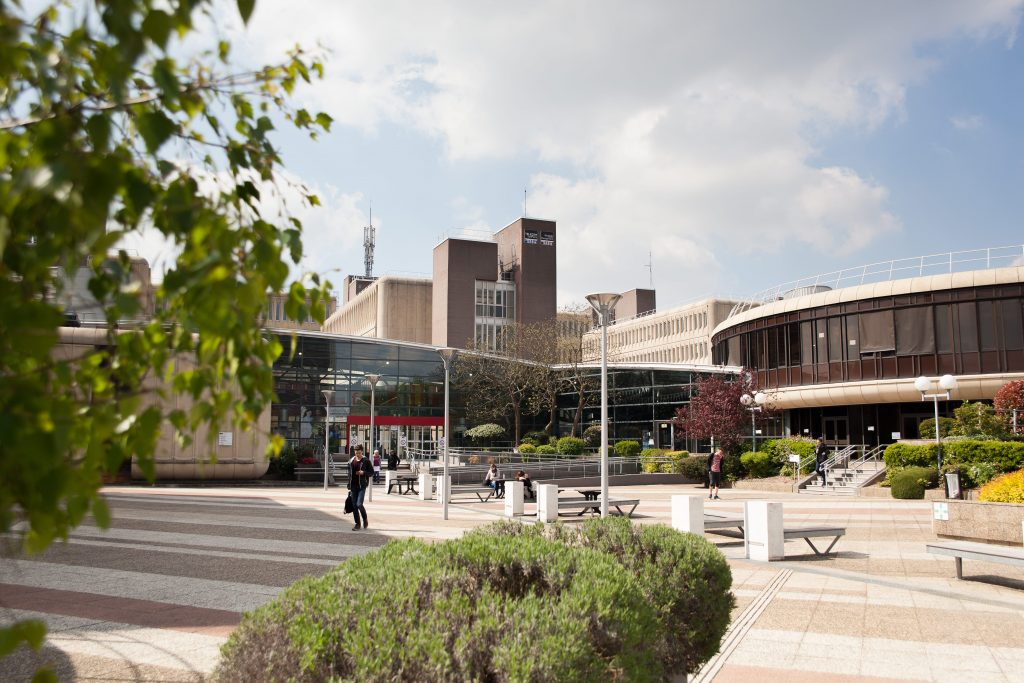
\includegraphics[width=0.7\textwidth]{img/campus_tsp.jpg}
    \caption{Photo du site}
    \label{fig:photo_site}
\end{figure}

%%%%%%%%%
%%%%%%%%%
%%%%%%%%%
%%%%%%%%%

\subsection{Service d'accueil}\label{ssec:introduction_service_accueil}

Ce stage a été encadré par \verb!François TRAHAY!, enseignant à \verb!Télécom SudParis! et chercheur au sein du laboratoire de recherche \verb!SAMOVAR! (Serivces répartis,\
Architectures, Modélisation, Validation, Administration des Réseux). Ce laboratoire accueille également quelques enseignants-chercheurs de l'\verb!ensIIE!, comme \verb!Valentin HONORÉ! qui a notamment co-encadré ce stage.\
Leurs travaux de recherche récents sont orientés vers l'analyse des performances dans le domaine du HPC (High Performance Computing).\
De plus, ils font partie de l'équipe \verb!BENAGIL! qui étudie la conception de systèmes distribués plus efficaces et plus sûrs en se focalisant sur leurs composants essentiels.

% TODO Présenter service/département de travail et son rôle dans entreprise
% On pourra aussi préciser le matériel à notre disposition pour mener notre stage

%%%%%%%%%
%%%%%%%%%
%%%%%%%%%
%%%%%%%%%

\subsection{Contexte et problématique}\label{ssec:introduction_contexte_problematique}

% TODO Présenter le contexte du stage et identifier les problèmes rencontrés qui justifient la pertinence du stage

%%%%%%%%%
%%%%%%%%%
%%%%%%%%%
%%%%%%%%%

\subsection{Objectifs du stage}\label{ssec:introduction_objectifs}

% TODO Présenter les objectifs du stage

%%%%%%%%%
%%%%%%%%%
%%%%%%%%%
%%%%%%%%%

\subsection{Contributions principales}\label{ssec:introduction_contributions}

% TODO Résumé des contributions majeures apportées

\newpage

%%%%%%%%%%%%%%%%%%%%%%%%%%%%%%%%
%%%%%%%%%%% CONTEXTE %%%%%%%%%%%
%%%%%%%%%%%%%%%%%%%%%%%%%%%%%%%%

\section{Contexte}\label{sec:contexte}

% -*- coding: utf-8 -*-
% !TEX root = ../main.tex

% TODO Présentation des travaux précédents pour expliquer d'où on part (programmes existants, études...)
% TODO Présenter les outils utilisés (logiciel/application, supercalculateur, langage de programmation...)
% Les sous-parties suivantes servent d'exemple, vous n'êtes pas obligés de les reprendre

\subsection{Concept du format de trace PALLAS}\label{ssec:pallas_status}

Les formats de trace classiques tels que \verb!OTF2! optimisent l'enregistrement et le compression de la trace mais ne permettent pas une factorisation réalisée lors de l'exécution du programme 
et ne ne permettent pas une macro-analyse efficace de la trace.\newline
Ainsi, \verb!PALLAS! sépare la trace en deux parties : l'une permettant une analyse structurelle de la trace et l'autre permettant un stockage précis des différents évènements.
Le poids total sur le disque est causé majoritairement par le stockage précis des évènements, donc le fait de stocker certaines informations plus "légères" séparément permet de ne pas 
avoir à charger la trace systématiquement pout toutes les analyses de cette dernière.\newline
Les évènements sont enregistrés par threads et stockés sous formes de tokens de manière hièrarchique : évènements, boucles et séquences.\newline
La détection des boucles est quant à elle en complexité $O(n^2)$ qui peut être bornée avec une longueur maximale, voire désactivée pour des applications trop irrégulières.

\subsubsection{Stockage hiérarchique des données}\label{ssec:hierarchy}

Il y a d'un côté les fichiers contenant tous les détails de l'exécution comme les durées et les timestamps de chaque évènement, regrouppés par token. \newline
De l'autre côté il y a un fichier beaucoup plus léger de structure qui permet d'avoir un résumé de la grammaire des tokens (évènements, séquences, boucles) ainsi que des statistiques
sur les différents données (durées minimales, maximales et moyennes). Ce fichier de structure permet de réaliser une macro-analyse rapide et efficace de la trace sans devoir charger toute la trace.\newline
Actuellement, l'écriture et la compression des données se fait en fin d'exécution. La compression par défaut est celle de l'algorithme \verb!ZSTD! qui est sans perte, mais d'autres sont 
proposés comme \verb!ZFP! qui sont avec perte. Un flush régulier pendant l'exécution serait également possible.

\subsubsection{Outils d'analyse fournis avec PALLAS}\label{ssec:analysis_tools}

Enfin, \verb!PALLAS! fournit des outils d'analyse de la trace déjà implémentés tels que: 
\begin{itemize}
    \item \verb!pallas_print! qui permet d'explorer toute la trace en l'affichant.
    \item \verb!pallas_contention! qui calcule le score de contention en utilisant uniquement les fichiers de structure (donc sans charger toute la trace).
    \item \verb!pallas_comm_matrix! qui réalise une matrice de communication MPI en n'utilisant également que la structure de la trace.
    \item \verb!pallas_histogram! qui extrait la distribution des durées grace à un accès précis aux vecteurs de durées concernés.
\end{itemize}

Le premier article \cite{pallas_ipdps} publié présentant \verb!PALLAS! montre que ces outils sont biens plus efficaces avec le format de trace \verb!PALLAS! que d'autres formats existants.

\subsection{Outils utilisés}\label{ssec:outils}

Les travaux réalisés lors de ce stage ont été mis en place sur la machine \verb!Sandor! de \gls{tsp}.
La machine \verb!Sandor! est un serveur de calcul équipé de deux processeurs physiques, 
offrant au total 64 c\oe{}urs et 128 threads.
Elle dispose de 504 \gls{go} de mémoire vive, ce qui en fait une plateforme adaptée aux charges de calcul intensives.\par
De plus, les applications \verb!MPI! utilisés comme benchmarks sont : LULESH et NAS BT, LU, MG, FT, CG, SP lancées sur 64 c\oe{}urs.

Les deux configuration utilisées sont : 
\begin{itemize}
    \item Vanilla : on exécute l'application sans outil de traçage
    \item \verb!EZTrace!/\verb!PALLAS! : on trace à l'aide de l'outil \verb!EZTrace! en utilisant le format de trace \verb!PALLAS!
\end{itemize}

Afin d'étudier la compression, on utilisera également le programme \verb!pallas_editor! qui permet de passer d'une trace compressée avec un algorithme A en une trace compressée avec
un algorithme B.

\newpage

%%%%%%%%%%%%%%%%%%%%%%%%%%%%%%%%
%%%%%%% TRAVAUX RÉALISÉS %%%%%%%
%%%%%%%%%%%%%%%%%%%%%%%%%%%%%%%%

\section{Travaux réalisés}\label{sec:travaux_realises}

% -*- coding: utf-8 -*-
% !TEX root = ../main.tex

% TODO Développer dans plusieurs sous-sections ce que vous avez réalisé pendant votre stage

\subsection{Organisation du repo pallas-analysis}\label{ssec:pallas_analysis_repo}

Le code ainsi que les graphiques réalisés lors de ce stage sont accessibles via le dépôt GitHub pallas-analysis \cite{pallas-analysis}.\newline
Ce dépôt regroupe les scripts \verb!bash! permettant d'installer et compiler \verb!PALLAS! avec \verb!EZTrace! ainsi que \verb!ZFP!, et des scripts 
\verb!python! permettant de réaliser les graphiques à partir des benchmarks lancés via des scripts \verb!bash!.
\newline
Ce dernier s'organise de la manière suivante :

\begin{figure}[!h]
\centering
\begin{minipage}{7cm}
\dirtree{%
.1 /pallas-analysis/.
    .2 analysis/.
        .3 prog/.
        .3 plot/.
        .3 results/.
    .2 build\_pallas\_eztrace/.
        .3 building\_eztrace\_pallas.sh.
        .3 setup\_all.sh.
    .2 run\_benchmarks/.
        .3 run\_nas\_benchmark/.
        .3 run\_lulesh/.
        .3 patches\_nas/.
        .3 divers scripts bash \( \ldots \).
    .2 Makefile.
    .2 README.md.
}
\end{minipage}
\caption{Arborescence de pallas-analysis}
\label{fig:dirtree}
\end{figure}

\subsection{Structure de données pour mesurer les performances}\label{ssec:clock}

Seulement le code de cette sous-partie est placé dans le dépôt GitHub de \verb!PALLAS! \cite{pallas-git} sur la branche \verb!nikolai!.
Voir l'annexe~\ref{ssec:details_durations} pour plus de détails.

Afin de mettre en place l'analyse des performances, on va utiliser la bibliothèque \verb!<time.h>! qui fournit une structure de temps (\verb!struct timespec!) avec
une composante en secondes et une composante en nanosecondes, ainsi qu'une fonction qui permet d'avoir le temps à un moment donné de l'exécution du code (\verb!clock_gettime!).\\

Ensuite, il y a une structure par bloc de code que l'on veut analyser avec les durées détaillées ainsi que les statistiques globales sur le bloc comme les durées totale, moyenne, minimale, maximale, ainsi que 
le nombre d'appels au bloc analysé et le temps total passé dans ce bloc.\\

Enfin, il y a une fonction permettant de mettre cette structure à jour à chaque appel au bloc de code que l'on souhaite analyser.\newline
Pour visualiser ces données on a des fonctions permettant d'écrire ces données sur le disque.

\subsection{Analyse du programme pallas\_print}\label{ssec:pallas_print}
\subsubsection{Positionnement du problème}\label{ssec:pallas_print_pbm}

La première tâche réalisée lors de ce stage a été l'analyse du programme pallas\_print qui permet d'afficher à l'écran une trace au format \verb!PALLAS!.
Pour ce faire, plusieurs points clés ont été analysés comme les différentes fonctions composant ce programme ainsi que la décomposition de certaines d'entre elles.

\begin{figure}[!h]
    \centering
    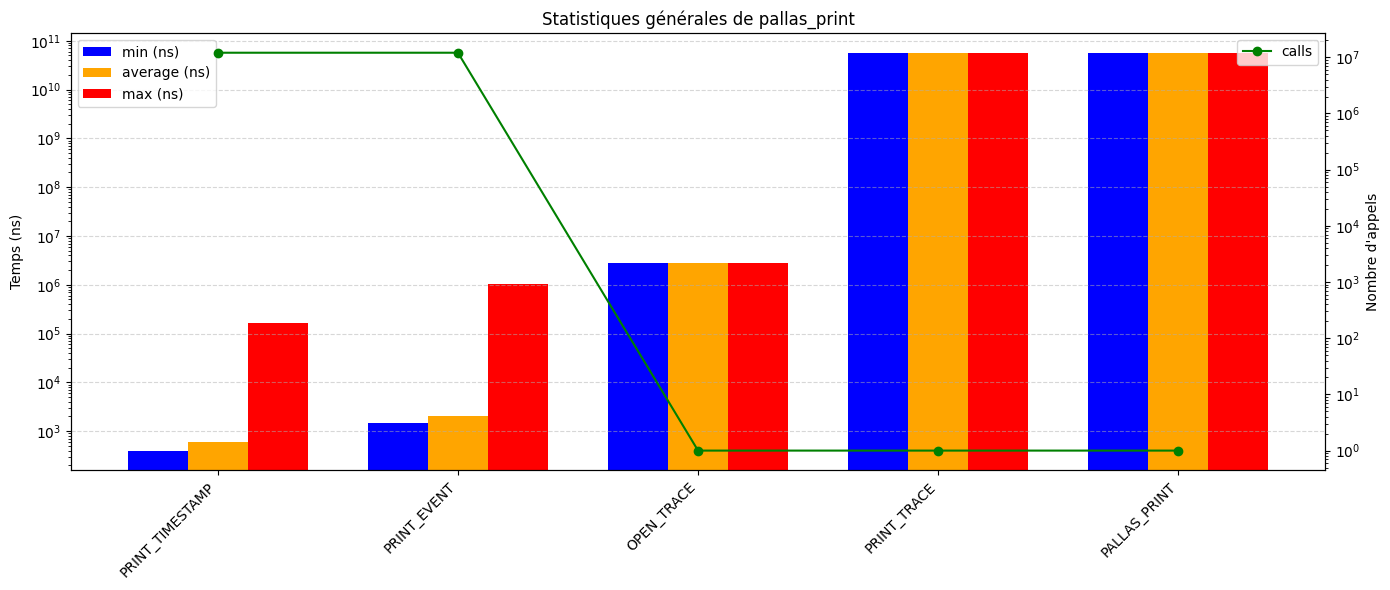
\includegraphics[width=1\textwidth]{img/pallas_print_gen.png}
    \caption{Statistiques générales de pallas\_print}
    \label{fig:pallas_print}
\end{figure}

Parmi les fonctions considérées, on a pallas\_print qui remprésente la durée totale de l'application, open\_trace qui est la durée d'ouverture de la trace,
puis print\_timestamp et print\_event qui sont les durées représentant respectivement l'affichage d'un timestamp et d'un évènement.
Le graphique ci-dessus~\ref{fig:pallas_print} a été réalisé sur une seule observation d'une trace issue du Benchmark NAS LU lancé sur 64 coeurs.

On remarque que la durée d'exécution totale de l'application pallas\_print est issue principalement de la fonction print\_event.

\subsubsection{Solution}\label{ssec:pallas_print_sol}

Ainsi, il faut analyser plus précisément la fonction print\_event.
Pour ce faire, j'ai découpé cette fonction en plusieurs parties. 

On remarque que, à chaque appel à cette fonction, il y a un appel à la fonction \verb!std::endl! de la bibliothèque standard C++. Or celle-ci réalise un flush systématique du buffer sur le disque.
Le fait de faire un flush systématique peut ajouter du temps inutile à l'exécution du programme.
Il est alors possible de remplacer ce \verb!std::endl! par l'écriture simple de \verb!'\n'!.


\begin{figure}[!h]
    \centering
    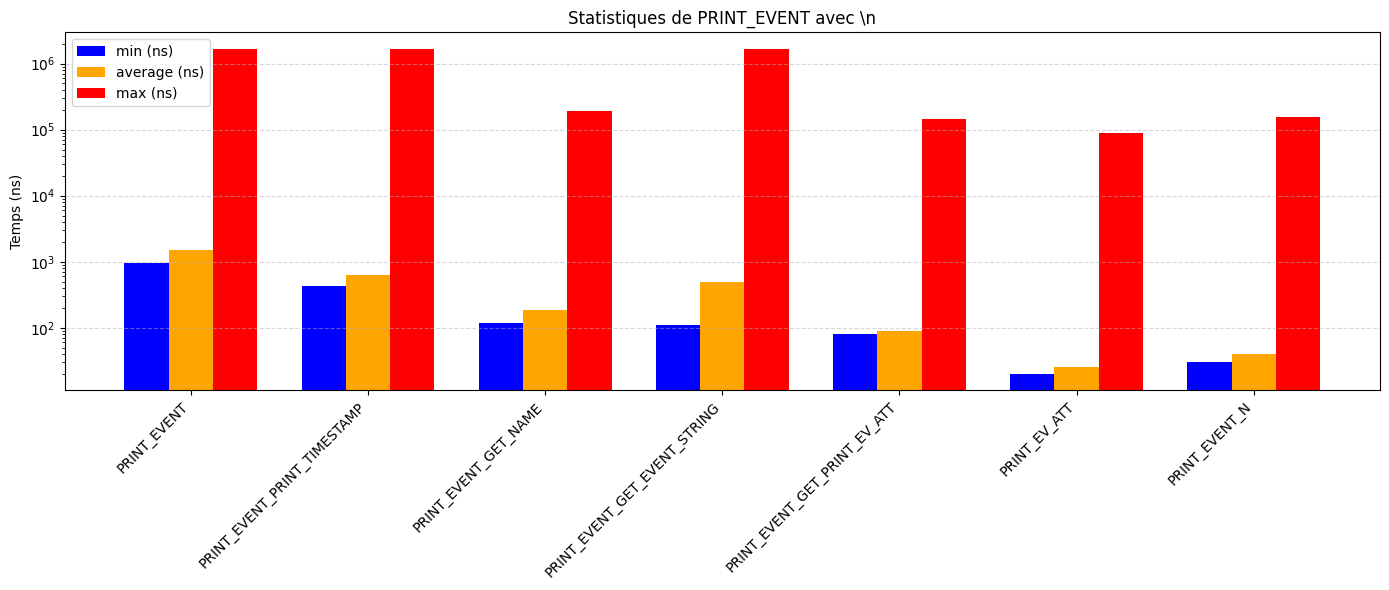
\includegraphics[width=1\textwidth]{img/print_event_n.png}
    \caption{Statistiques détaillées de print\_trace avec un '\textbackslash n'}
    \label{fig:print_event_n}
\end{figure}

\begin{figure}[!h]
    \centering
    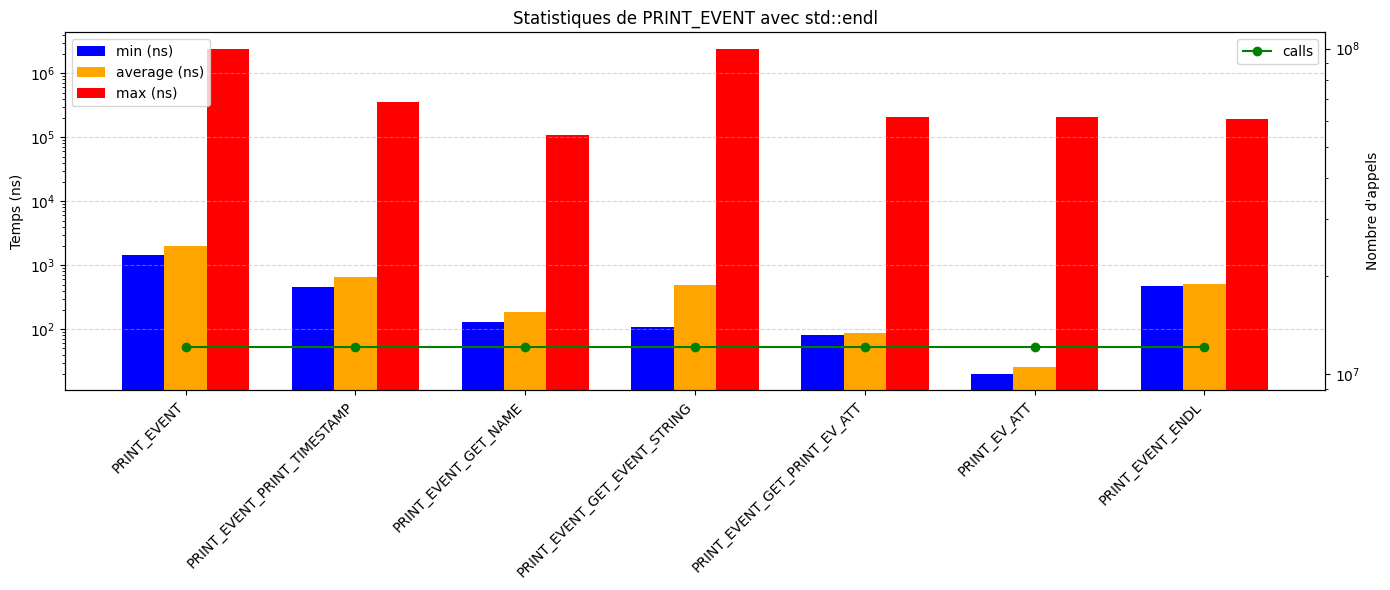
\includegraphics[width=1\textwidth]{img/print_event_endl.png}
    \caption{Statistiques détaillées de print\_trace avec un std::endl}
    \label{fig:print_event_endl}
\end{figure}

Ainsi, sur la figure~\ref{fig:print_event_n} on observe les statistiques de print\_trace avec l'écriture d'un \verb!'\n'! et sur la figure~\ref{fig:print_event_endl} on a les statistiques de print\_trace avec un \verb!std::endl!.
Cette trace ayant 12067968 évènements, on passe d'un temps total par appel à print\_trace à 2000 ns/évènement avec un \verb!std::endl! à 1500 ns/évènement avec l'écriture de \verb!'\n'!, ce qui représente un gain
total de 500 ns/évènement, et dans le cas de cette trace 6 secondes sur le temps d'exécution total.\\
Enfin, c'est une application difficile à analyser et à optimiser car il y a un certain nombre de données à charger avec des copies de structures de dictionnaire.


\subsection{Evaluation de l'overhead induit par PALLAS}\label{ssec:overhead}
\subsubsection{Mise en situation}\label{ssec:overhead_context}

Dans le contexte du calcul haute performance, il est primordial d'utiliser des outils dont l'impact est minimal sur les performances des applications.
C'est ce que l'on va essayer d'évaluer pour l'utilisation de \verb!PALLAS! dans cette partie.

Tout d'abord, il a fallu mettre en place des outils afin de réaliser cette évaluation. Ces outils seront réutilisés dans toute la suite de l'analyse et sont tous dans le repo \cite{pallas-analysis}.

Afin d'installer \verb!PALLAS! avec le traceur \verb!EZTrace!, il y a le script \verb!building_eztrace_pallas.sh! situé dans le dossier \verb!build_pallas_eztrace/!.
Puis, pour lancer les différents benchmarks, il y a les scripts \verb!bash! situés dans le dossier \verb!run_benchmarks! permettant de compiler les différents
exécutables dans un premier temps, puis de lancer les programmes dans un second temps (de plusieurs manières différentes, en fonction des données que l'on veut récupérer et de l'aspect que l'on souhaite étudier).

Dans le cadre de l'étude de l'overhead (temps ajouté au programme initial par l'utilisation de \verb!PALLAS!), on a besoin de récupérer principalement la durée totale de l'exécution du programme.
Pour ce faire, j'ai utilisé la commande \verb!time! de Linux.

\subsubsection{Protocole expérimental}\label{ssec:overhead_exp}

Afin d'analyser l'overhead de manière précise, il a fallu exécuter tous les benchmarks présentés dans la partie~\ref{ssec:outils} de ce rapport, avec et sans \verb!EZTrace!.
Ces benchmarks ont été itérés 20 fois pour plus de précision.

De plus, il a fallu récupérer ces données d'exécution dans les fichiers de log de ces derniers et enfin les tracer à l'aide de la bibliothèque \verb!matplotlib! de \verb!Python!.
Afin d'uniformiser les barres relatives à chaque application, les valeurs de ces dernières ont normalisées par les données de l'application Vanilla (sans tracé).

\subsubsection{Résultats}\label{ssec:overhead_res}

\begin{figure}[!h]
    \centering
    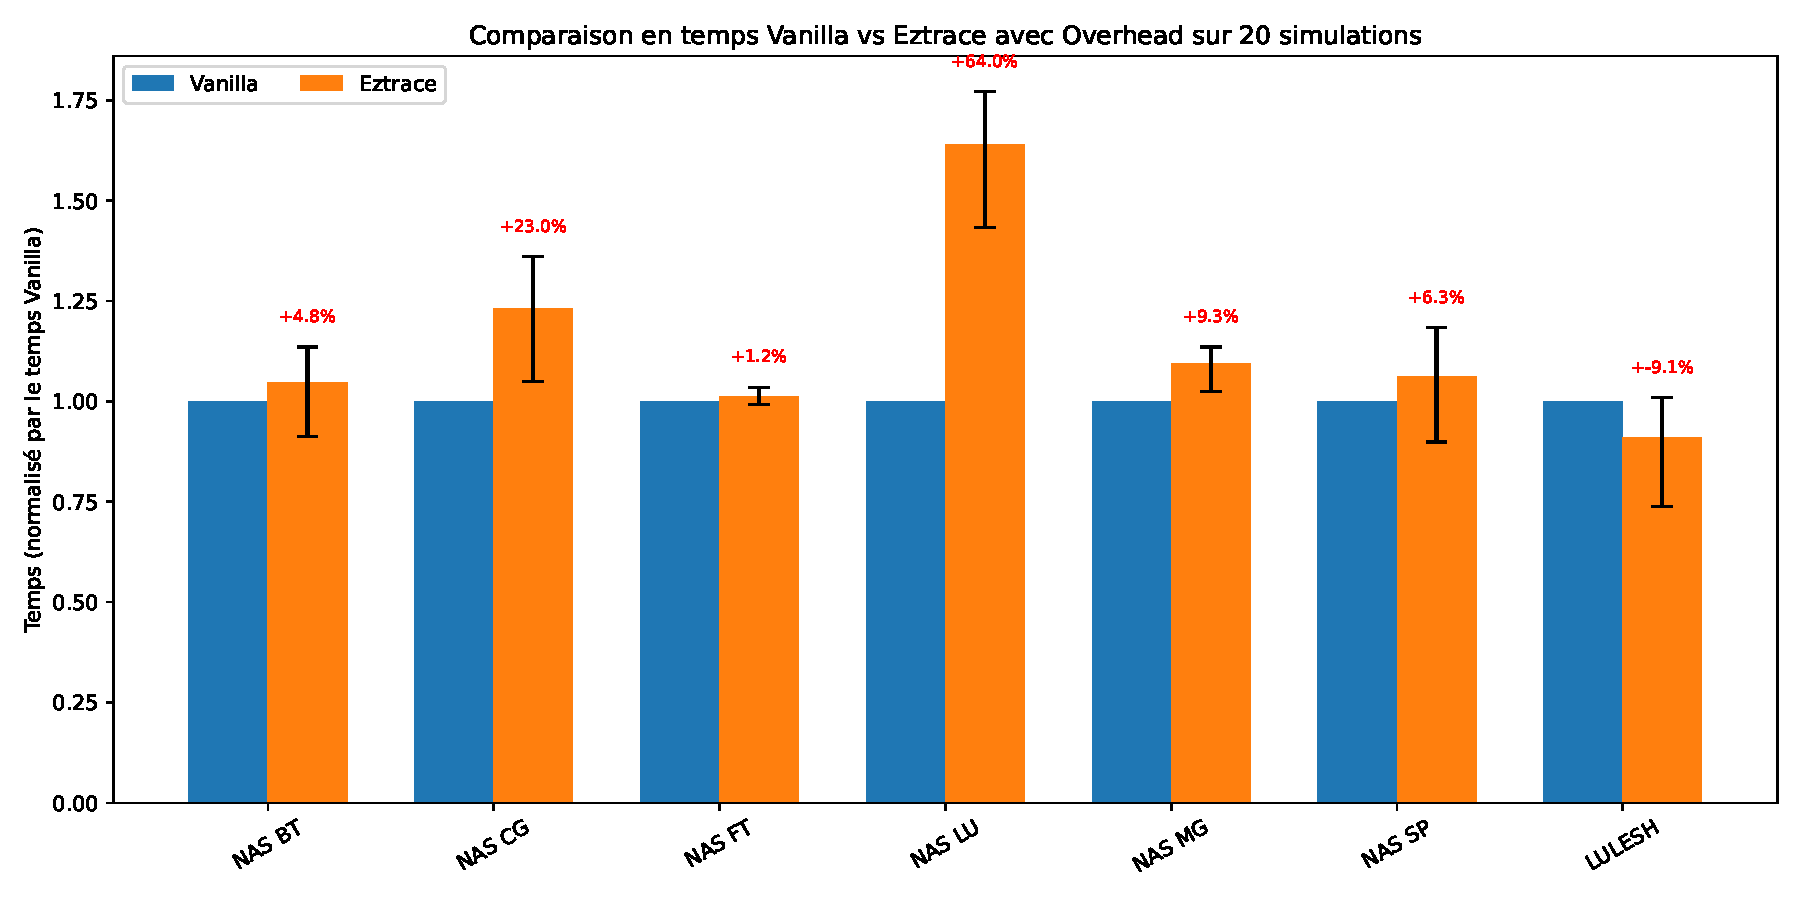
\includegraphics[width=1\textwidth]{img/overhead.pdf}
    \caption{Overhead généré par EZTrace/PALLAS}
    \label{fig:overhead}
\end{figure}

Les résultats de l'overhead induit par le tracé de \verb!EZTrace! sont représentés dans le graphique~\ref{fig:overhead}.
On constate que dans les cas comme \verb!NAS BT!, \verb!NAS FT!, \verb!NAS MG!, \verb!NAS SP! et \verb!LULESH!, on a un impact inférieur à 10\% du temps total d'exécution de l'application.
Dans les cas des benchmarks \verb!NAS BT! et surtout \verb!NAS LU! on a un impact significatif sur le temps d'exécution total de l'application qui atteint un maximum de 64\%.
Ainsi, on peut conclure que dans les cas d'applications très régulières, l'overhead induit par l'utilisation de \verb!PALLAS! avec \verb!EZTrace! reste suffisament négligeable.

\subsection{Analyse de la compression et de l'écriture sur les disque de PALLAS}\label{ssce:wrt_write}

\subsubsection{Situation actuelle}\label{ssec:wrt_situ}

\verb!PALLAS! enregistre les différentes données d'exécution sous forme de listes doublement chainées, décomposées en sous-listes dont la taille est fixée.
Tout le vecteur est stocké en mémoire et écrit d'un seul coup sur les disques en fin d'exécution.
L'algorithme de compression retenu par défaut est \verb!ZSTD! qui est un algorithme sans pertes.

\subsubsection{Methodes d'analyse}\label{ssec:wrt_analysis}

Un facteur intéressant à faire varier est la taille des sous-vecteurs permettant de stocker les données. Par défaut, celle-ci est fixée à \verb!1000!.
Afin, de les faire varier, j'ai appliqué des patchs git (qui permettent d'enregistrer différents commits) à la taille de ces sous-vecteurs.
Les tailles testées sont \verb!100!, \verb!1000!, \verb!10000!, \verb!100000!, \verb!500000!, \verb!1000000!.
Les données recueillies sont les statistiques sur le temps d'écriture et de compression (par fonctions puis par parties de fonctions) lors de l'exécution
d'un programme avec différentes tailles de vecteurs.
Puis des graphiques sont réalisés grace à des scprits \verb!python! qui permettent d'aggréger les données. 

\subsubsection{Résultats obtenus}\label{ssec:wrt_res}

\begin{figure}[!h]
    \centering
    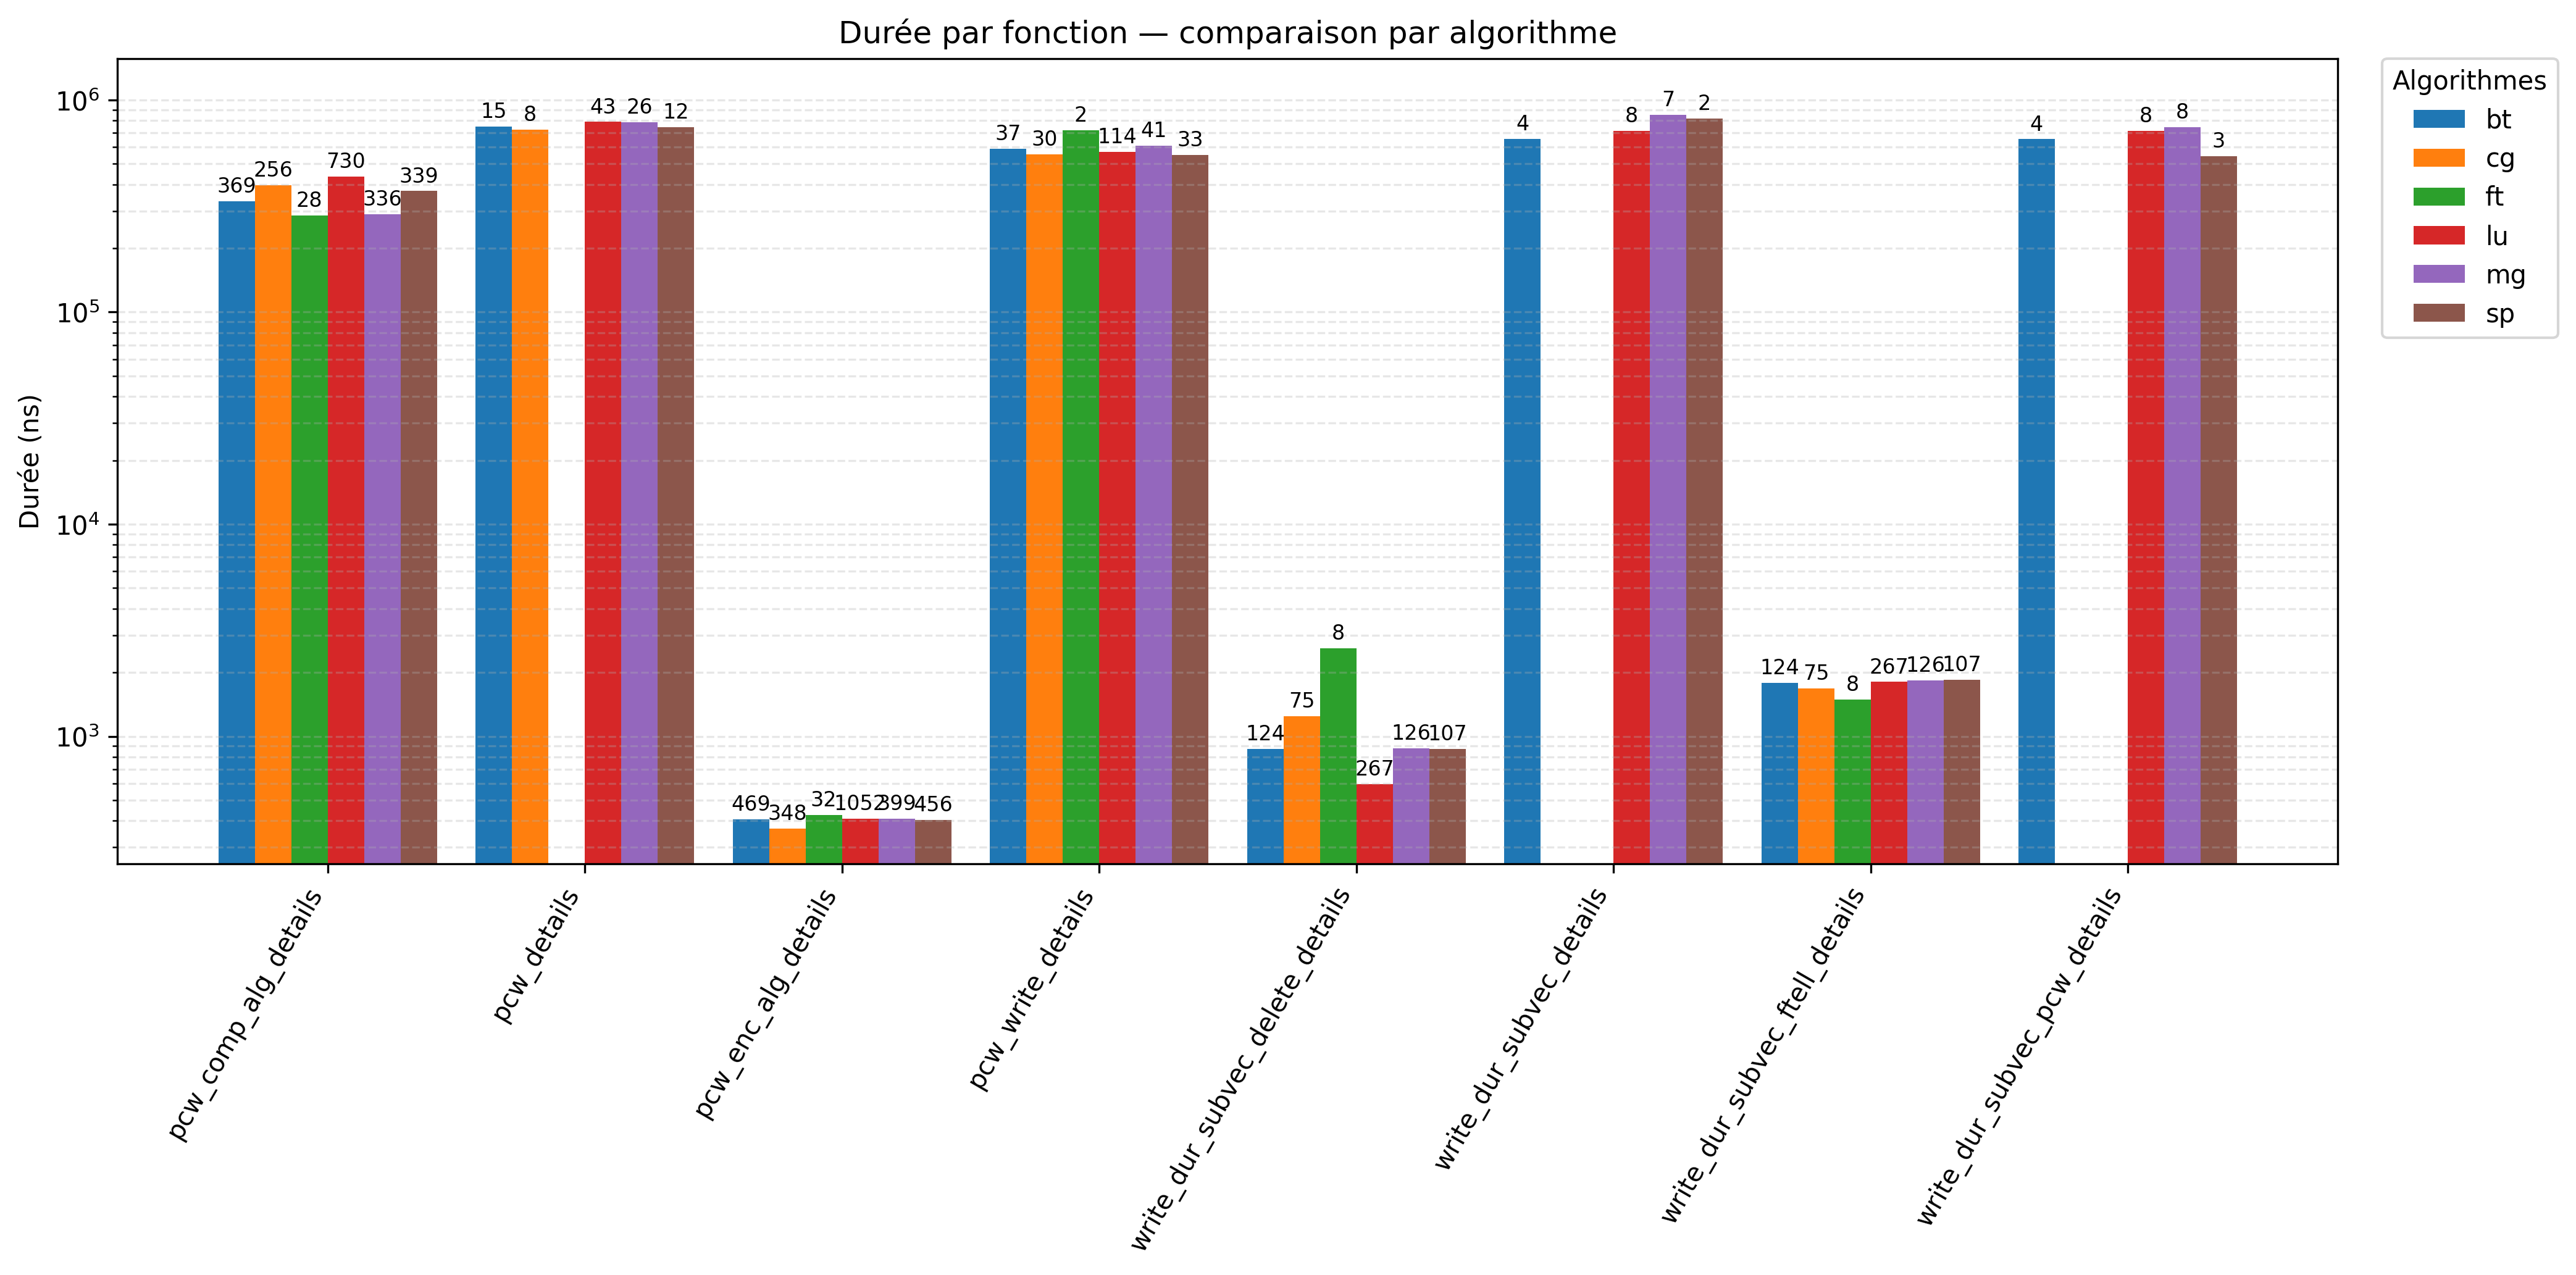
\includegraphics[width=1\textwidth]{img/pcw_global.png}
    \caption{Durées générales de l'écriture et de la compression}
    \label{fig:pcw_global}
\end{figure}
\begin{figure}[!h]
    \centering
    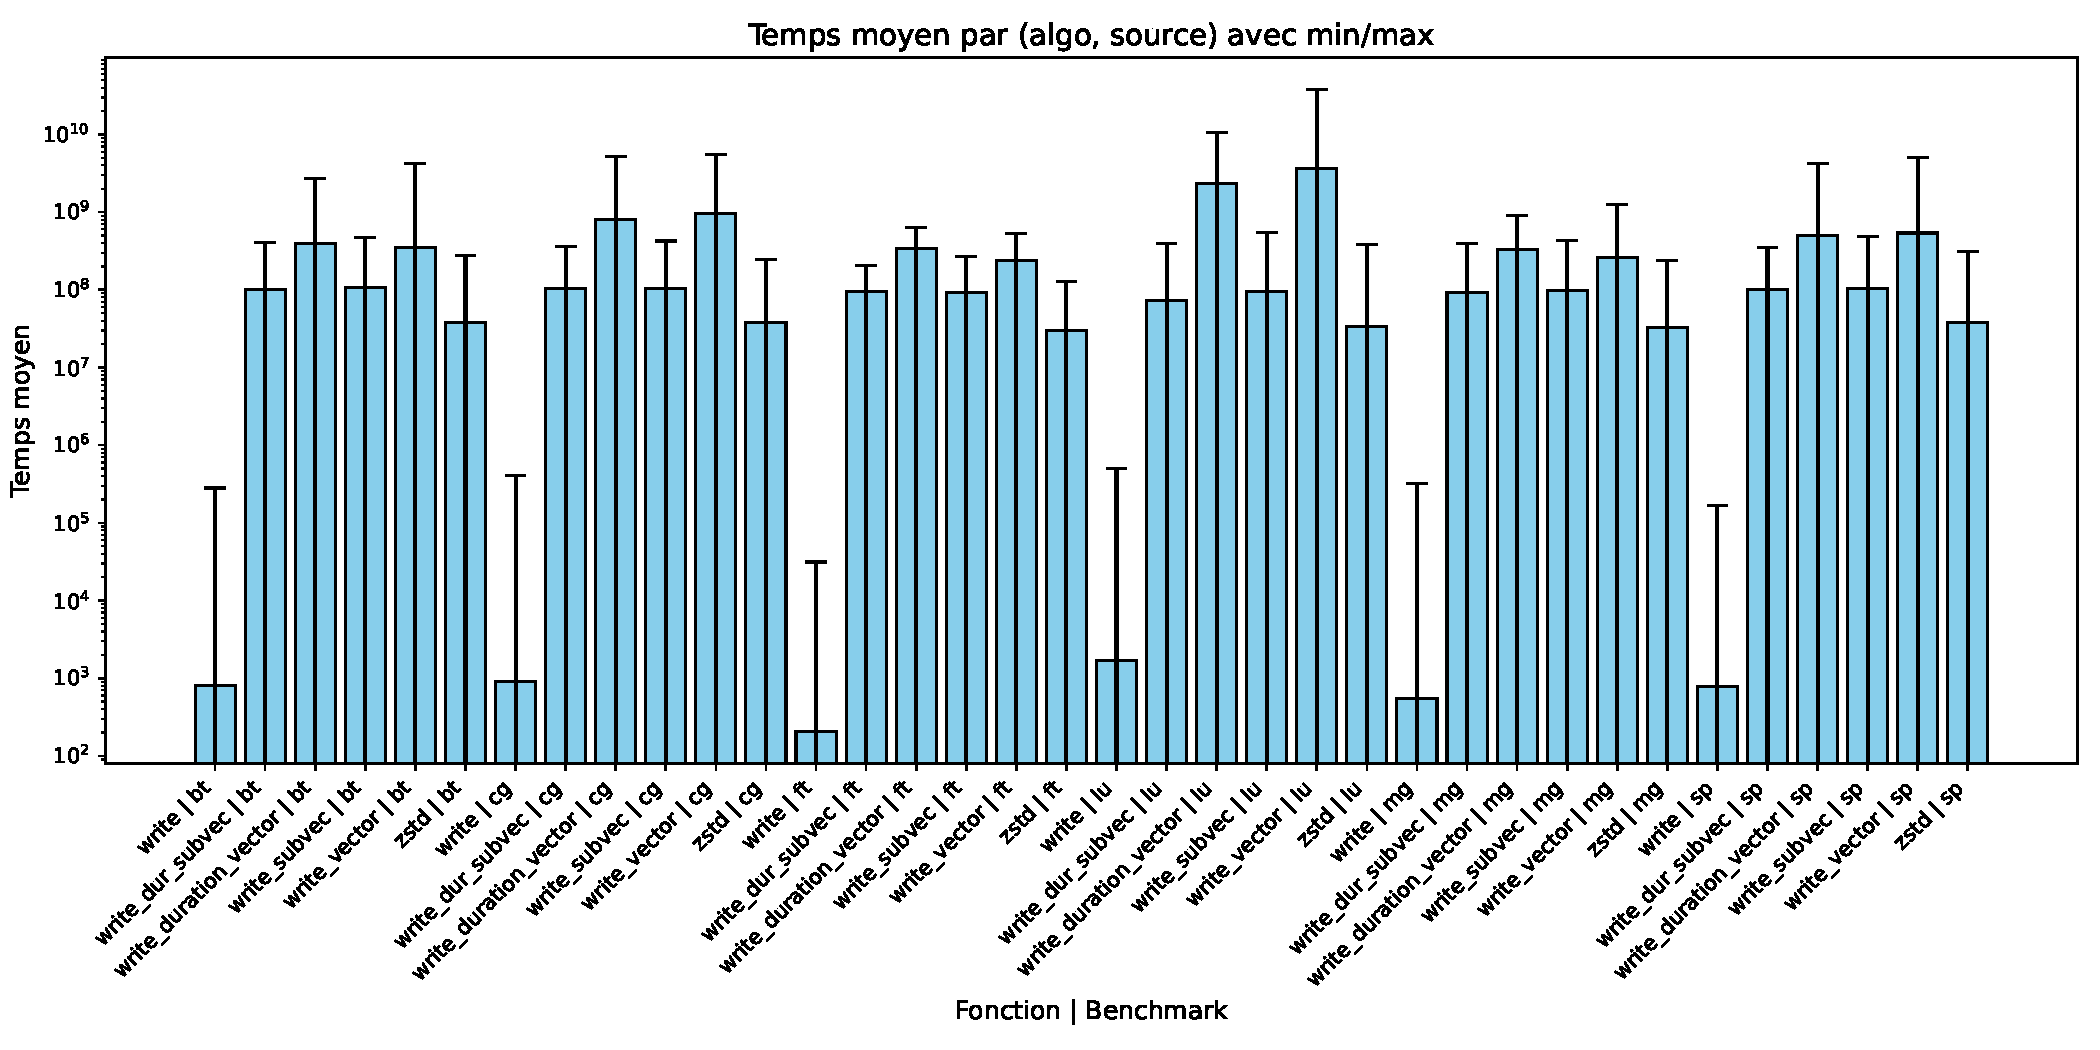
\includegraphics[width=1\textwidth]{img/nas_comp_write.pdf}
    \caption{Fonctions d'écriture et de compression}
    \label{fig:cw_global}
\end{figure}
Tout d'abord, l'écriture sur le disque ainsi que la compression des données sont réalisés par la fonction \verb!pallas_compress_write! (abrégé par pcw dans le graphique~\ref{fig:pcw_global}),
donc avant de lancer les programmes sur différentes tailles de sous-vecteurs, il faut observer cette fonction là.
Le nombre d'appels à chaque fonction dans chacun des benchmarks est écrit au dessus de chaque barre.\\
On remarque que le temps total de la fonction de compression et d'écriture est dû principalement à la fonction d'écriture ainsi que celle de compression.

De plus, d'après le graphique~\ref{fig:cw_global}, on observe que ce sont les fonctions \verb!write_vector! et \verb!write_duration_vector! (qui écrivent respectivement les vecteurs de timestamps et de durées)
qui prennent le plus de temps.\\
\begin{figure}[!h]
    \centering
    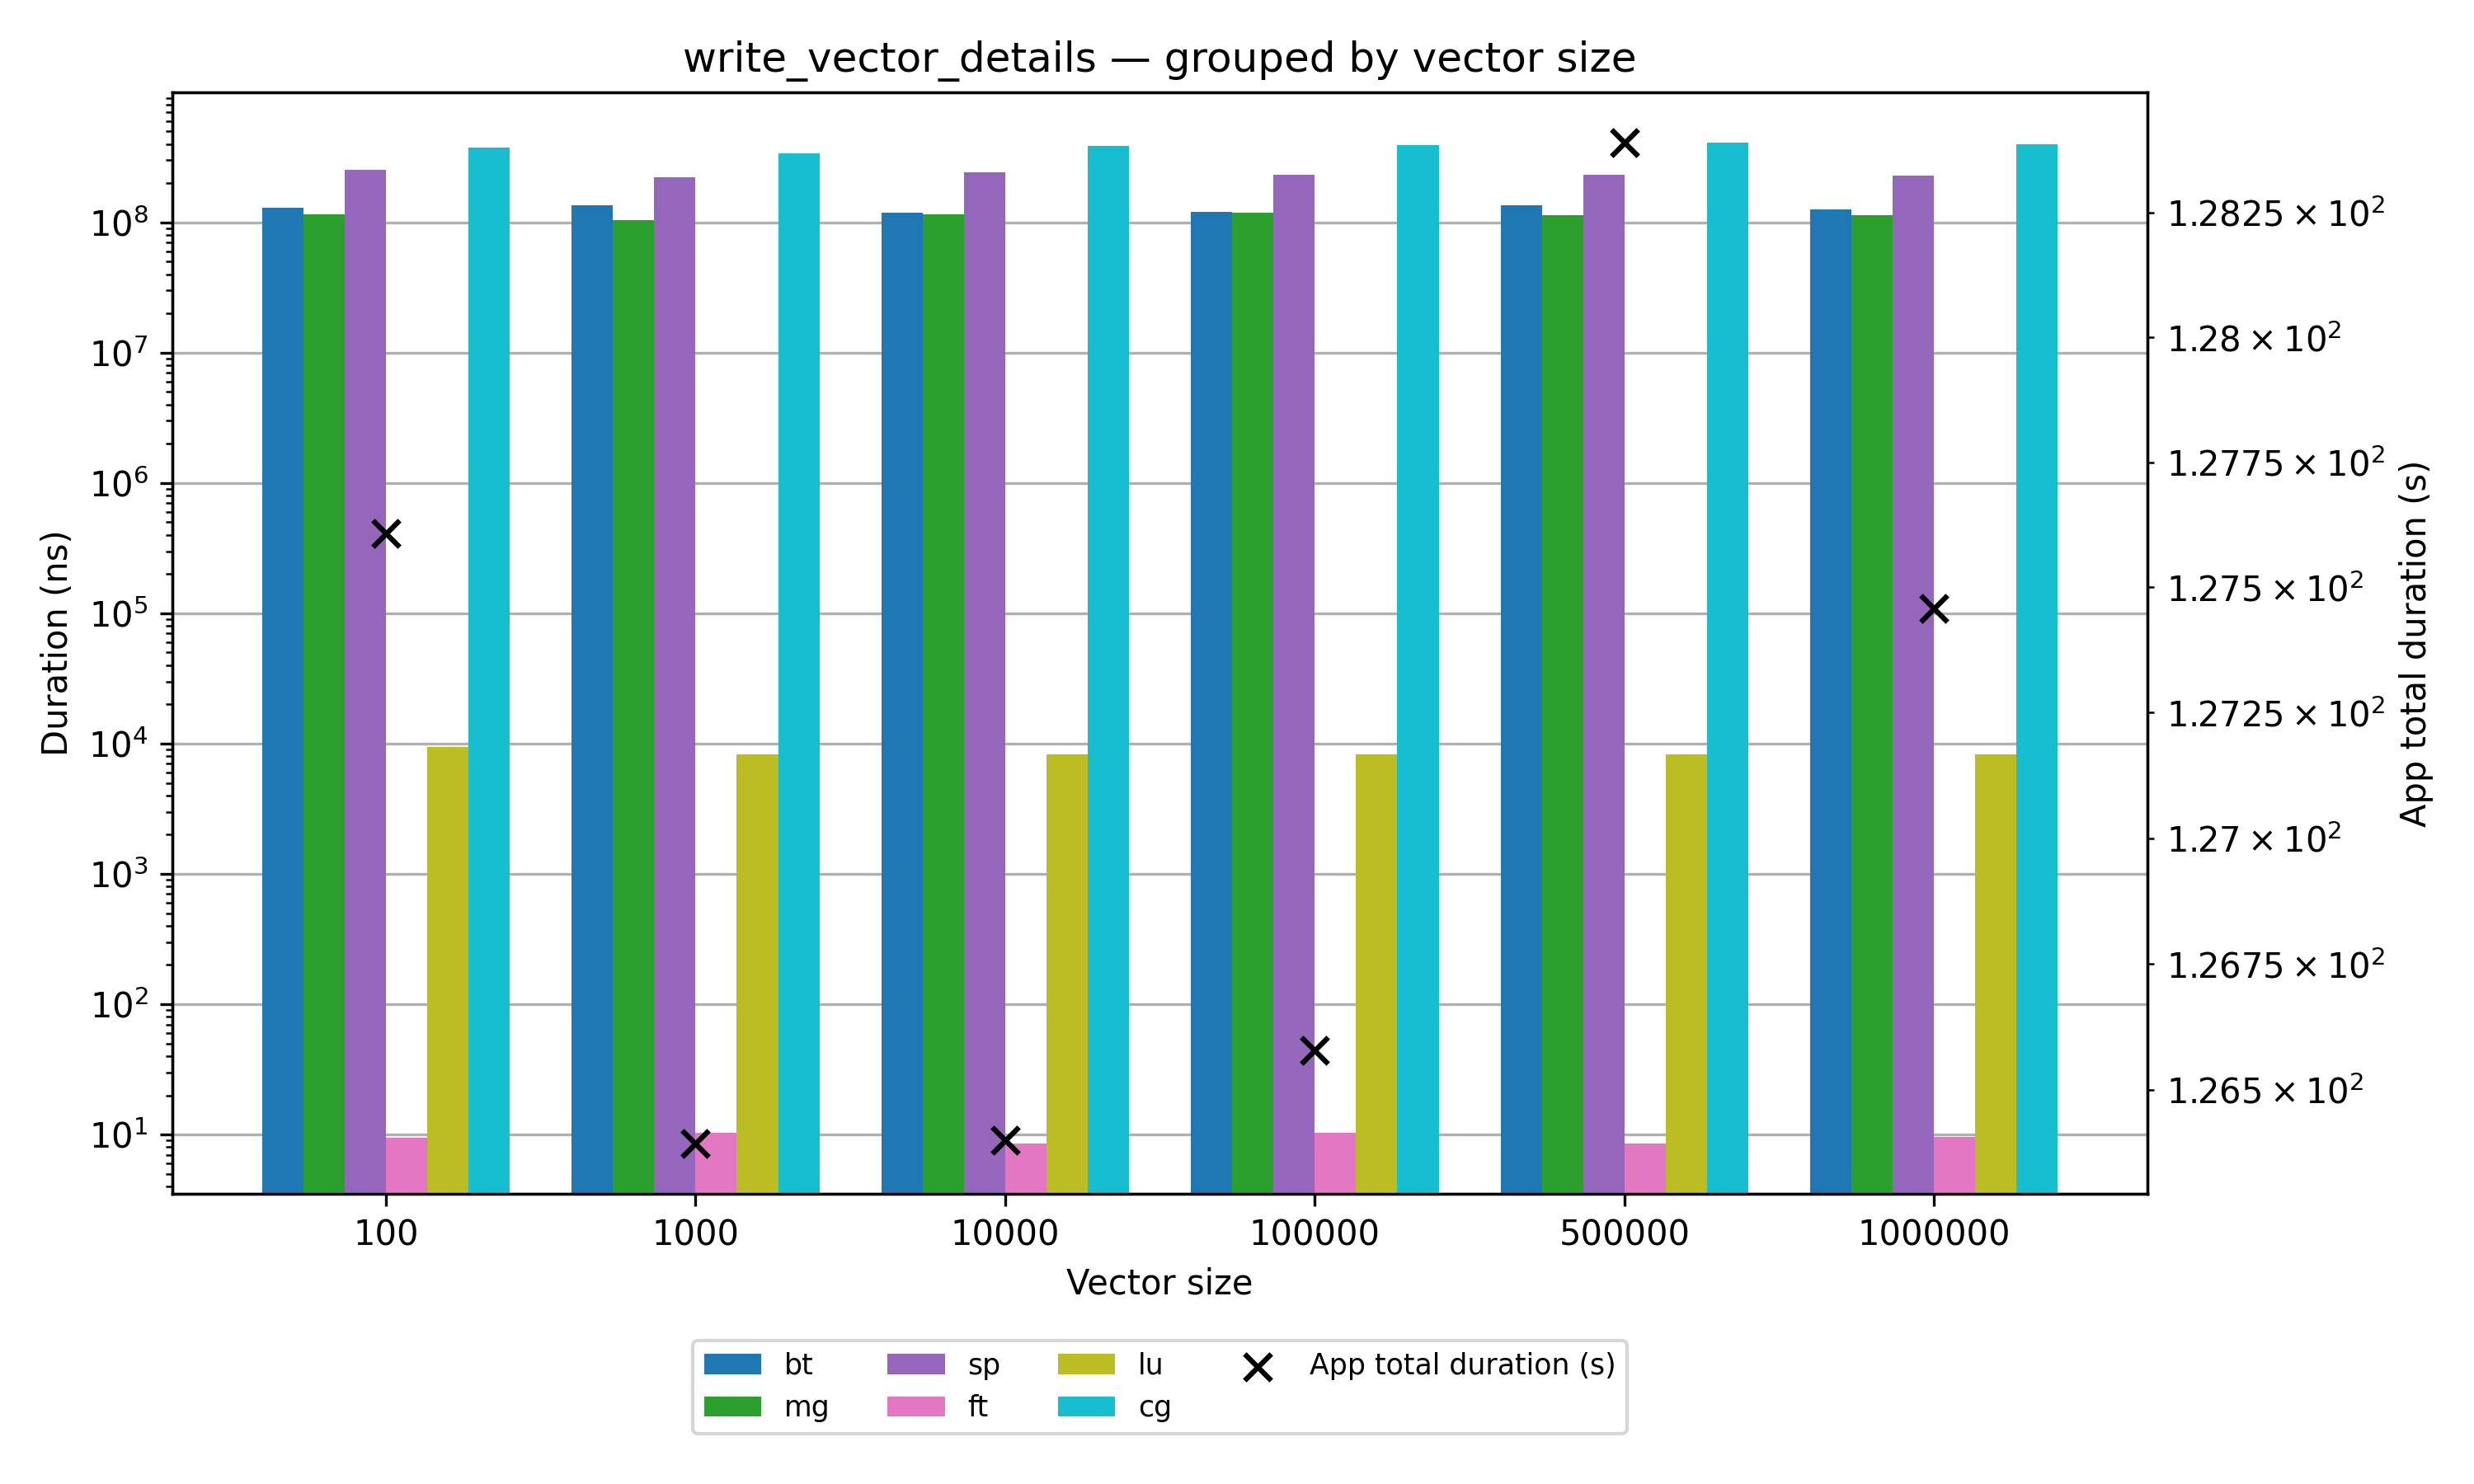
\includegraphics[width=1\textwidth]{img/write_vector_details.png}
    \caption{Statistiques des durées de l'écriture d'un vecteur}
    \label{fig:a}
\end{figure}
\begin{figure}[!h]
    \centering
    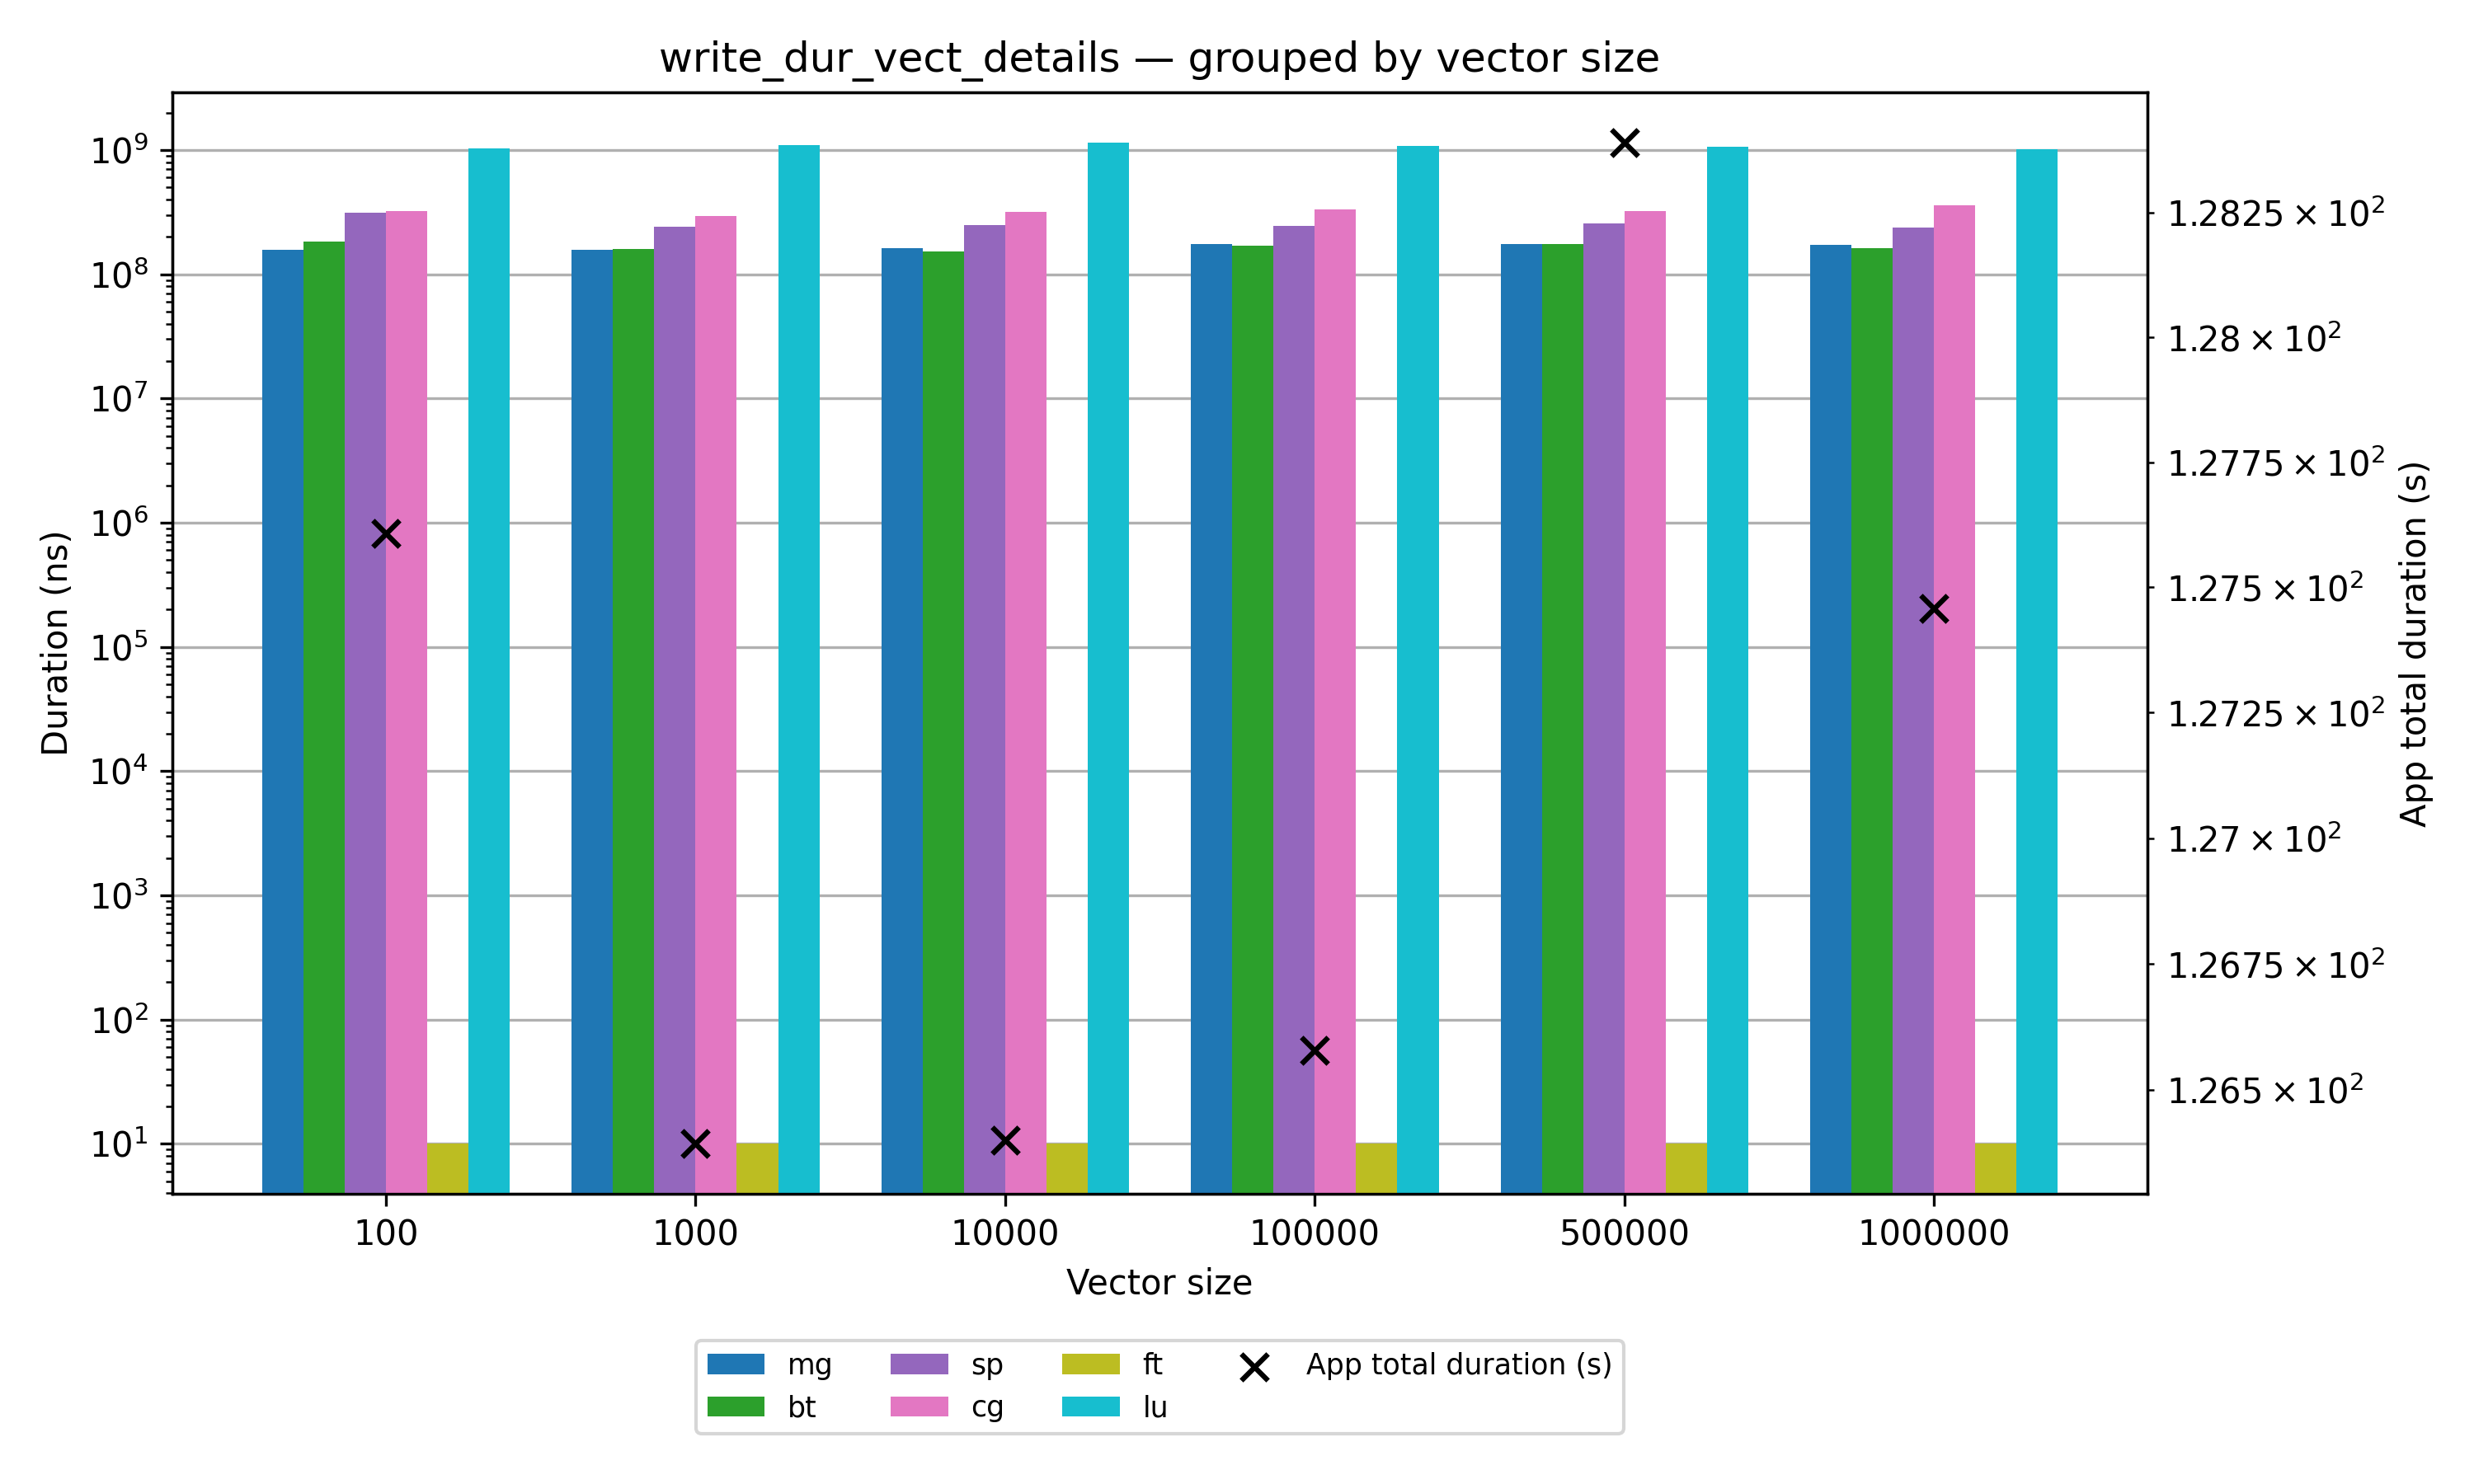
\includegraphics[width=1\textwidth]{img/write_dur_vect_details.png}
    \caption{Statistiques des durées d'écriture d'un vecteur de durées}
    \label{fig:b}
\end{figure}
\begin{figure}[!h]
    \centering
    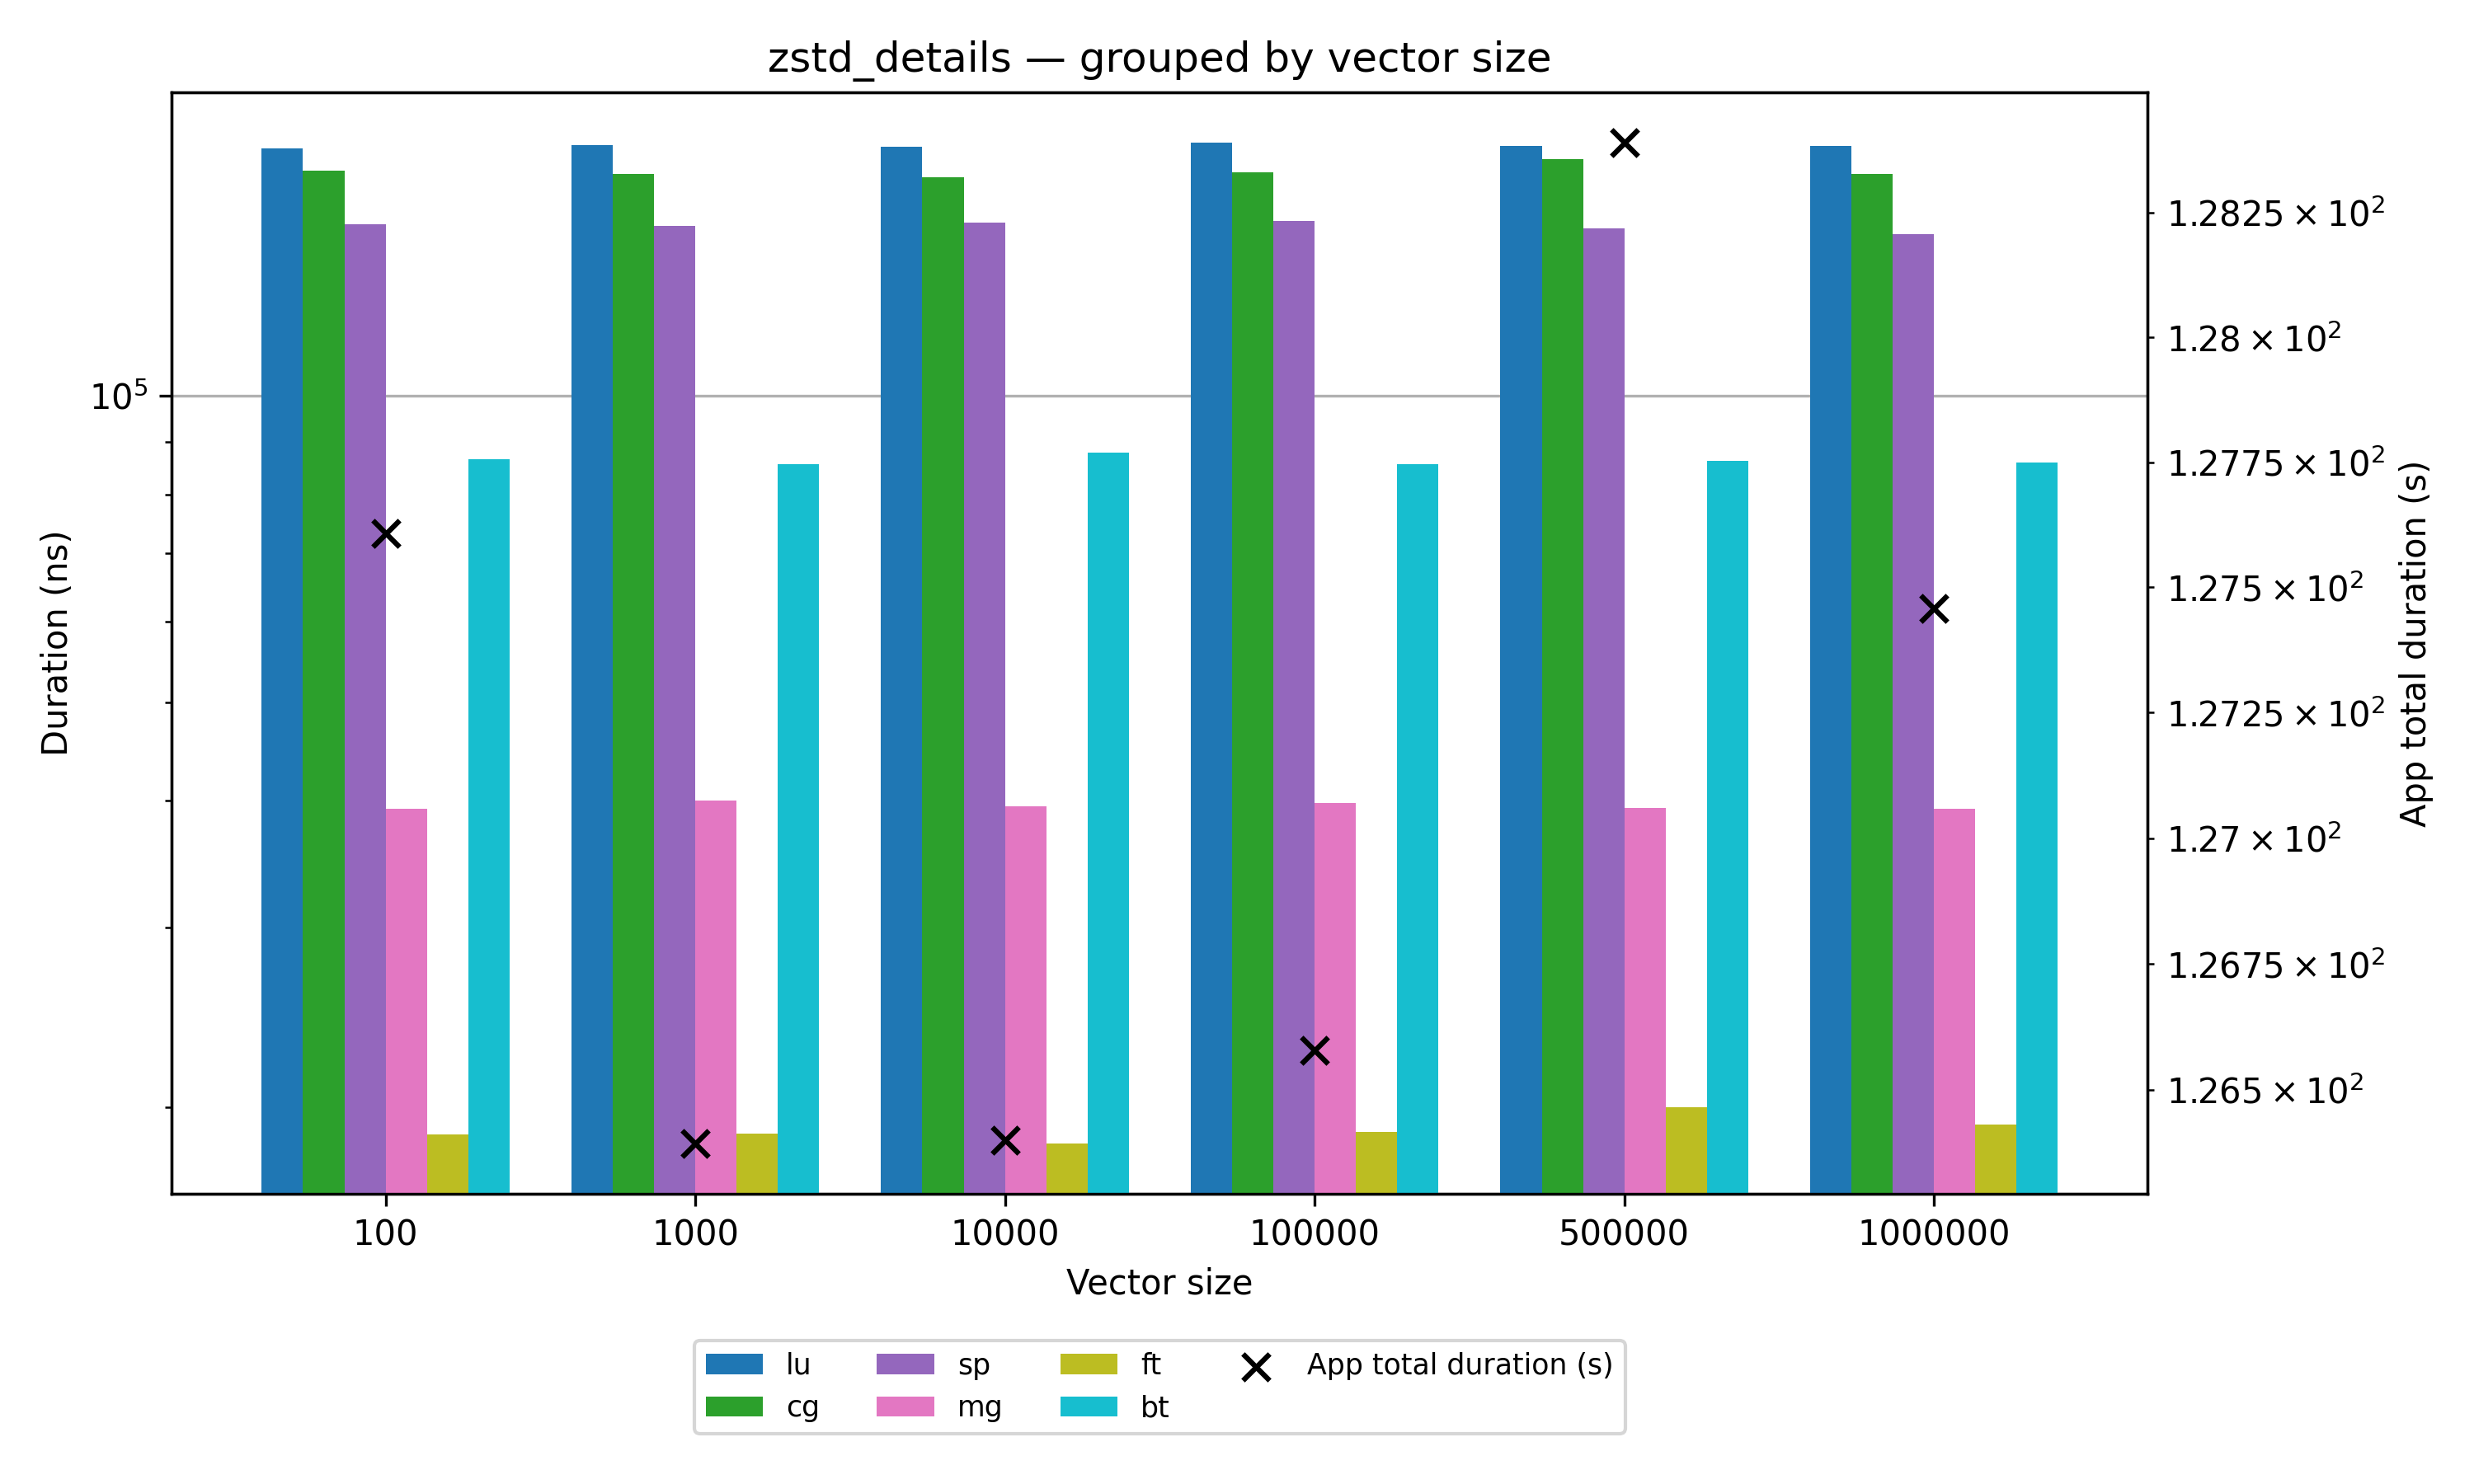
\includegraphics[width=1\textwidth]{img/zstd_details.png}
    \caption{Statistiques de durée de la compression d'un vecteur}
    \label{fig:c}
\end{figure}
\begin{figure}[!h]
    \centering
    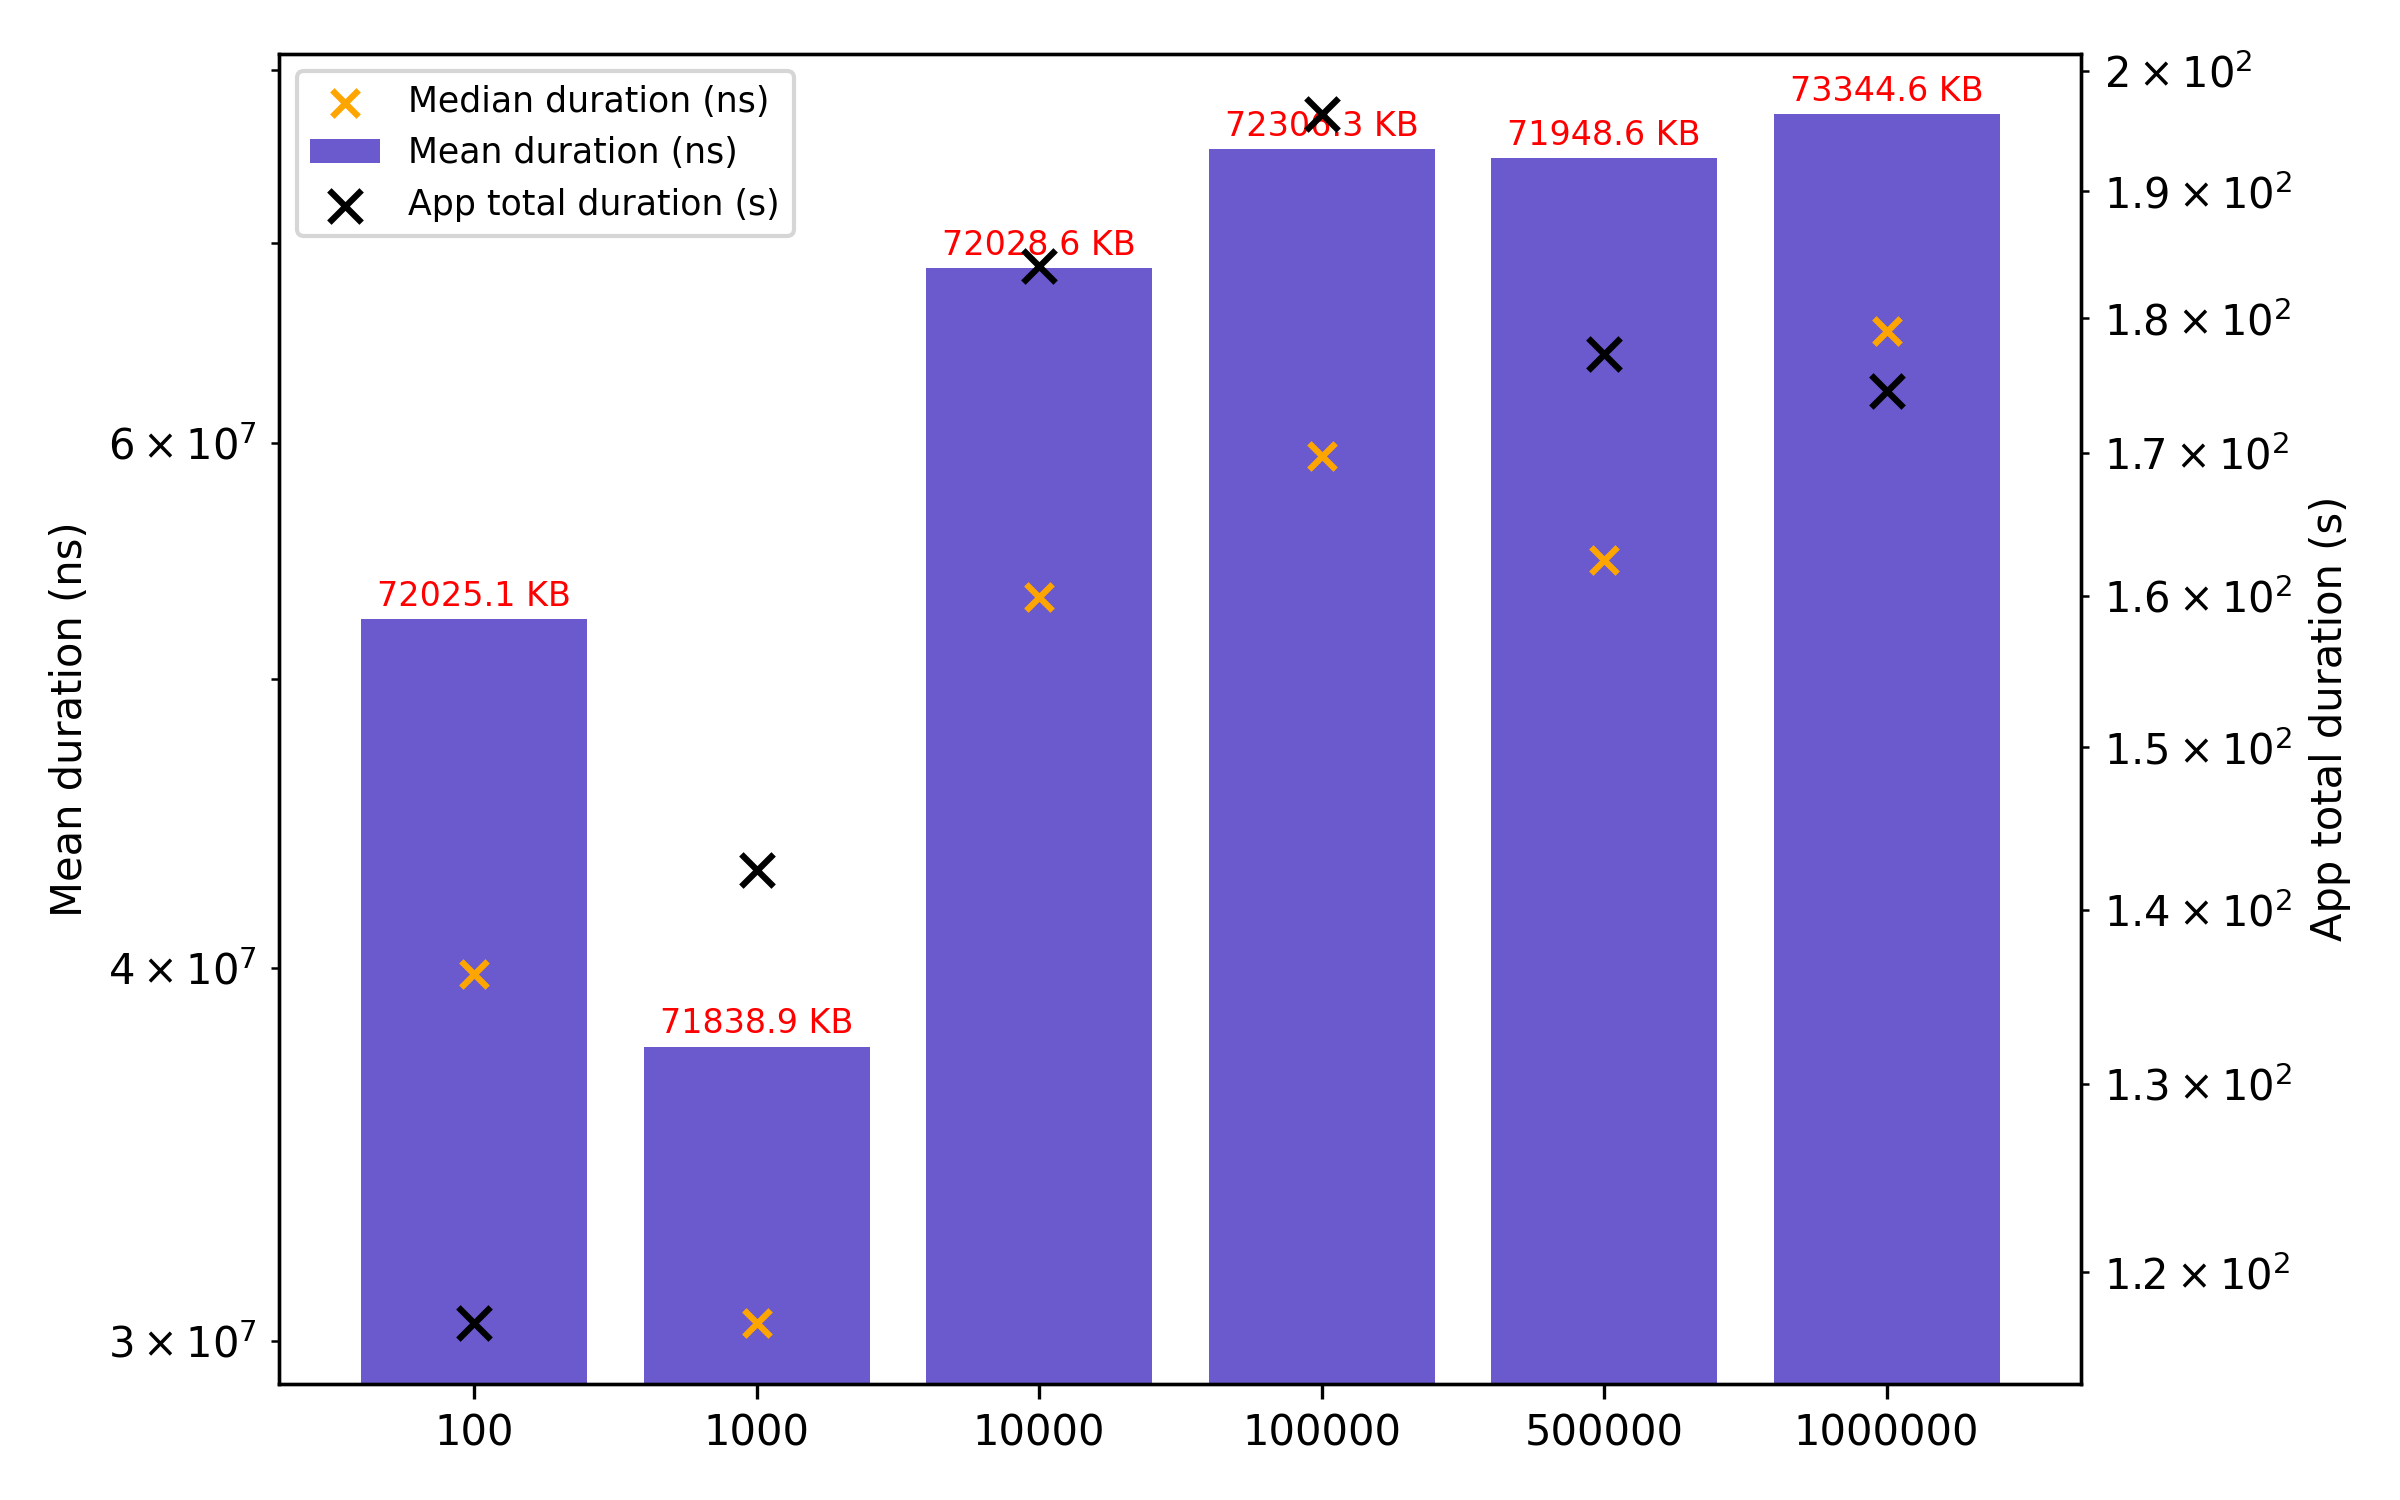
\includegraphics[width=1\textwidth]{img/write_dur_subvec_bof.png}
    \caption{Moyennes des durées d'écriture d'un vecteur de durées}
    \label{fig:d}
\end{figure}
Dans le graphique~\ref{fig:d}, une moyenne a été réalisée sur toutes les applications observées par taille de sous-vecteur et par fonction observée (ici l'écriture d'un vecteur de durées a été observée).
On remarque alors que c'est pour une taille de sous-vecteur de \verb!1000!, c'est-à-dire la longueur par défaut que l'on a les meilleurs résultats. 
En rouge, on observe également le pic mémoire lors des différentes exécutions, qui est assez stable mais minime pour la taille de \verb!1000!.
Mais ce graphique est à relativiser car une moyenne non pondérée a été faire alors que les différentes traces ont des tailles extrêmement variées.

Enfin, pour la comparaison des comportements des fonctions les plus coûteuses en fonction de la taille des sous-vecteurs (écriture et compression de ces derniers),
on retrouve les résultats dans les graphiques~\ref{fig:a},~\ref{fig:b} et~\ref{fig:c}.

On observe alors que la variation des tailles de sous-vecteurs n'a pas un impact marquant sur ces fonctions. Par contre, grâce aux croix noires sur ces graphiques qui représentent le temps d'exécution total du programme,
on constate que la taille des sous-vecteurs a tout de même un impact sur le temps d'exécution total (de l'ordre de 2 secondes pour les application observées).

Au final, même si la taille des sous-vecteurs n'a pas un grand impact sur l'application, la taille fixée à \verb!1000! semble être optimale.


\clearpage


\subsection{Etude de différents algorithmes de compression}\label{ssec:comp}
\subsubsection{Situation actuelle}\label{ssec:comp_situ}

L'algorithme de compression choisi par défaut est \verb!ZSTD! qui est sans perte, c'est-à-dire qu'il garantit une restitution parfaite des données, sans erreurs.
Mais \verb!PALLAS! propose d'autres algorithmes tels que \verb!ZFP! qui sont "lossy", c'est-à-dire avec une certaine proportion de perte autorisée.
L'objectif est d'évaluer la perte d'information de ces algoritmes ainsi que leur efficacité.

\subsubsection{Outils mis en place}\label{ssec:comp_tools}

La problématique dans le fait d'évaluer la perte d'information liée à différents algorithmes a été la mise en place d'un outil permettant cette étude.
La solution retenue a été de générer une trace avec \verb!EZTrace! et \verb!PALLAS! et d'utiliser l'application \verb!pallas_editor! qui permet, à partir d'une trace
existante, d'en créer une nouvelle avec un autre algorithme de compression. Ainsi, on peut comparer des traces identiques avec des algorithmes de compression différents.

En suite, les applications \verb!pallas_getTimestamps! et \verb!pallas_durations! ont été mises en place. La première permet de récupérer, à partir d'une trace, un fichier \verb!.csv! avec 
tous les timestamps de cette dernière, récupérés thread par thread. La seconde réalise le test statistique $R^2$ sur deux échantillons de timestamps (la version sans compression sert d'échantillon
de référence).

Ces des applications n'ont pas pu être regrouppées en une seule car l'architecture actuelle de \verb!PALLAS! ne permet pas de parcourir deux fois la même trace de cette manière 
(une partie de ce problème a été résolue car initialement il était impossible d'ouvrir deux traces différentes au même endroit).

\subsubsection{Résultats obtenus}\label{ssec:comp_res}

Les données récoltées ont été classées dans les tables~\ref{lu},~\ref{bt} et \ref{cg} et permettent comparer les différents algorithmes de compression pour les quelques benchmarks considérés
(\verb!NAS LU!, \verb!NAS BT! et \verb!NAS CG!).
Les différents algorithmes de compression étudiés sont l'absence de compression (\verb!None!), \verb!ZSDT!, et l'algorithme \verb!ZFP! avec plusieurs seuils de tolérence différents 
(\verb!0.1!, \verb!0.2!, \verb!0.3!).

% ---------- LU ----------
\begin{table}[h]
\centering
\caption{Résultats LU}\label{lu}
\begin{adjustbox}{max width=\linewidth}
\begin{tabular}{lrrrrr}
\hline
\textbf{Valeur} & \textbf{None} & \textbf{ZSTD} & \textbf{ZFP\_0.1} & \textbf{ZFP\_0.2} & \textbf{ZFP\_0.5} \\
\hline
$R^2$                     & 1            & 1            & 1             & 1             & 1 \\
trace\_size\_MB           & 168          & 67           & 93            & 93            & 93 \\
compression\_duration\_ns & 0            & 1.84647e+09  & 1.48667e+09   & 1.50095e+09   & 1.52376e+09 \\
write\_duration\_ns       & 2.61871e+08  & 1.56096e+08  & 1.90319e+08   & 1.98531e+08   & 1.96283e+08 \\
\hline
\end{tabular}
\end{adjustbox}
\end{table}

% ---------- BT ----------
\begin{table}[h]
\centering
\caption{Résultats BT}\label{bt}
\begin{adjustbox}{max width=\linewidth}
\begin{tabular}{lrrrrr}
\hline
\textbf{Valeur} & \textbf{None} & \textbf{ZSTD} & \textbf{ZFP\_0.1} & \textbf{ZFP\_0.2} & \textbf{ZFP\_0.5} \\
\hline
$R^2$                     & 1           & 1           & 1            & 1            & 1 \\
trace\_size\_MB           & 105         & 46          & 60           & 60           & 60 \\
compression\_duration\_ns & 0           & 1.14903e+09 & 8.90252e+08  & 8.96525e+08  & 8.87341e+08 \\
write\_duration\_ns       & 1.7996e+08  & 9.39251e+07 & 1.07688e+08  & 1.13053e+08  & 1.16274e+08 \\
\hline
\end{tabular}
\end{adjustbox}
\end{table}

% ---------- CG ----------
\begin{table}[h]
\centering
\caption{Résultats CG}\label{cg}
\begin{adjustbox}{max width=\linewidth}
\begin{tabular}{lrrrrr}
\hline
\textbf{Valeur} & \textbf{None} & \textbf{ZSTD} & \textbf{ZFP\_0.1} & \textbf{ZFP\_0.2} & \textbf{ZFP\_0.5} \\
\hline
$R^2$                     & 1           & 1           & 1            & 1            &  \\
trace\_size\_MB           & 161         & 57          & 84           & 84           & 84 \\
compression\_duration\_ns & 0           & 1.61676e+09 & 1.42368e+09  & 1.444e+09    & 1.41518e+09 \\
write\_duration\_ns       & 2.4251e+08  & 1.29261e+08 & 1.75401e+08  & 2.0416e+08   & 1.66534e+08 \\
\hline
\end{tabular}
\end{adjustbox}
\end{table}

On constate alors que pour tous les algorithmes, le test $R^2$ vaut \verb!1! (à 12 chiffres significatif près), ce qui signifie que les échantillons sont assez proches pour être considérés comme identiques.
De plus, la taille de la trace non compressée vaut environ le double de celle de la trace compressée avec l'algorithme \verb!ZSTD!. Pour ce qui est de \verb!ZFP!, la taille est entre les deux (plus proche 
de la trace compressées avec \verb!ZSTD! tout de même).
Pour ce qui est du temps de compression de la trace, il est plus long pour l'algorithme \verb!ZSTD! que pour l'algorithme \verb!ZFP!, mais cette différence se compense avec le
temps d'écriture qui est au contraire plus long pour l'algorithme \verb!ZSTD!. L'écriture de la trace non compressée dure quasiment aussi longtemps que les temps d'écriture et de 
compression additionnés pour \verb!ZSTD! ou \verb!ZFP!.

Au final, il semble plus judicieux d'utiliser, dans le cas général, l'algorithme \verb!ZSTD! car celui-ci permet de réduire drastiquement la taille de la trace (environ de moitié)
sans pour autant ajouter du temps au programme de manière significative ni compromettre l'intégrité des données (ce qui est au final le cas pour chacun des algorithmes étudiés).
\newpage

%%%%%%%%%%%%%%%%%%%%%%%%%%%%%%%%
%%%%%% RÉSULTATS OBTENUS %%%%%%%
%%%%%%%%%%%%%%%%%%%%%%%%%%%%%%%%

\section{Résultats obtenus}\label{sec:resultats_obtenus}

% -*- coding: utf-8 -*-
% !TEX root = ../main.tex

% TODO Présentation de vos résultats

\newpage

%%%%%%%%%%%%%%%%%%%%%%%%%%%%%%%%
%%%%%%%%%% CONCLUSION %%%%%%%%%%
%%%%%%%%%%%%%%%%%%%%%%%%%%%%%%%%

\section{Conclusion et perspectives}\label{sec:conclusion}

% -*- coding: utf-8 -*-
% !TEX root = ../main.tex

\subsection{Conclusion}\label{ssec:conclusion_conclusion}

Ce stage m'as permis de faire le tour de plusieurs points clés du fonctionnement de \verb!PALLAS!.
En effet, j'ai pu, dans un premier temps, afin de prendre en main les outils nouveaux, étudier le fonctionnement d'une application très utile en pratique, \verb!pallas\_print!.
Dans un second temps, j'ai eu pu étudier l'impact général du tracé avec \verb!EZTrace! au format \verb!PALLAS! sur le programme.
Enfin, j'ai vérifié des points clés de l'écriture sur les disques avec une étude de la tailles des sous-vecteurs ainsi que de la compression des données en étudiant différents algorithmes 
de compression proposés par \verb!PALLAS!, tant sous l'aspect de la perte d'information que sur leurs impacts sur le temps total d'exécution du programme.

%%%%%%%%%
%%%%%%%%%
%%%%%%%%%
%%%%%%%%%

\subsection{Retours d'expérience}\label{ssec:conclusion_retours}

% TODO Vos retours d'expérience : ce que vous avez appris/découvert

A travers ce stage j'ai pu mettre en application beacoup des outils appris lors de ma première année à l'école, comme la programmation impérative et orientée objet, ainsi que 
l'utilisation du \verb!shell! et le scripting avec \verb!bash! qui m'as permis d'automatiser beaucoup de tâches ainsi que de récupérer aisément différentes données liées 
à l'exécution de différents programmes.
De plus, j'ai beaucoup appris à travers l'utilisation de programmes nouveaux comme \verb!screen! qui permet de lancer des programmes et pouvoir se "détacher"
du processus concerné. De plus, j'ai appris l'utilisation de la bibliothèque \verb!time! qui permet d'avoir très facilement des données liées au temps dans un programme. Côté, \verb!python!
j'ai appris à utiliser différentes bibliothèques comme par exemple \verb!matplotlib! ou \verb!pandas! pour récupérer et aggréger des données puis les visualiser.

De plus, ce stage m'as permis de découvrir le monde de la recherche. En effet, j'ai pu apprendre à travailler en autonomie sur des sujets demandant des prises d'initiative, tout en étant 
encadré par des enseignants qui ont su me guider au mieux tout au long de ce stage, avec 
parfois le besoin de mettre en place de nouveaux outils (comme avec \verb!pallas\_durations!). Le cadre de \verb!Télécom SudParis!, quant à lui, m'as permis d'échanger au quotidien 
avec des enseignants-chercheurs ainsi que des doctorants et en apprendre plus sur leur travail. Enfin, j'ai eu l'occasion d'assister à une soutennace de thèse, ce qui m'as 
donné un apperçu de la finalité du travail des doctorants que j'ai côtoyé.

%%%%%%%%%
%%%%%%%%%
%%%%%%%%%
%%%%%%%%%

\subsection{Perspectives}\label{ssec:conclusion_perspectives}

% TODO Les perspectives d'amélioration ou d'utilisation de votre programme/de ce que vous avez développé

Tout d'abord, j'aurais apprécié avoir le temps de mettre en place et d'évaluer le flush progressif sur les disques des différents sous-vecteurs pendant l'exécution, et non d'un seul coup à la fin de celle-ci.\\
De plus, il serait intéressant de fixer le bug à cause duquel il n'est pas possible de parcourir deux fois les données d'une trace (l'équipe avait déjà reglé le fait qu'il était impossible 
d'ouvrir deux traces dans un même programme, ce qui pouvait être problématique pour de futures analyses de traces).

%%%%%%%%%
%%%%%%%%%
%%%%%%%%%
%%%%%%%%%

\newpage

%%%%%%%%%%%%%%%%%%%%%%%%%%%%%%%%
%%%%%%%%%%%%% DDRS %%%%%%%%%%%%%
%%%%%%%%%%%%%%%%%%%%%%%%%%%%%%%%

\appendix
\section{Développement durable et responsabilité sociétale}\label{sec:ddrs}

% -*- coding: utf-8 -*-
% !TEX root = ../main.tex

% TODO Annexe DDRS

%%%%%
%%%%%
%%%%%

\subsection{Développement durable}

Un exemple sympa. \cite{cea-terathermie}

%%%%%
%%%%%
%%%%%

\subsection{Responsabilité sociétale}

\newpage

%%%%%%%%%%%%%%%%%%%%%%%%%%%%%%%%%%%%
%%% ORGANISATION DE L'ENTREPRISE %%%
%%%%%%%%%%%%%%%%%%%%%%%%%%%%%%%%%%%%

\section{Organisation de l'entreprise}\label{sec:organisation}

% -*- coding: utf-8 -*-
% !TEX root = ../main.tex

% TODO Organigrammes de l'entreprise pour comprendre comment l'entreprise est structurée



\begin{figure}[ht]
\small
\noindent\textbf{T\'el\'ecom SudParis — Organigramme (version listes, noms inclus)}\\[2pt]

\textbf{Direction}
\begin{itemize}\itemsep2pt
  \item Directeur — Fran\c{c}ois Dellacherie
  \item Directeur adjoint — Herv\'e Debar
\end{itemize}

\textbf{Directions m\'etiers}
\begin{itemize}\itemsep2pt
  \item Formations — Dir. : Emmanuel Monfrini
  \item Relations internationales — Dir. int. : St\'ephane Maag
  \item Recherche et formations doctorales — Dir. : Herv\'e Debar
  \item Innovation et Relations Entreprises — Dir. : Olivier Martinot
  \item Communication — Dir. : Sandrine Bourguer
  \item Affaires g\'en\'erales — D\'el\'egu\'e : Benoit Jean
\end{itemize}

\textbf{D\'epartements d'enseignement et de recherche}
\begin{itemize}\itemsep2pt
  \item ARTEMIS — Dir. : Titus Zaharia 
  \item CITI — Dir. : Randal Douc
  \item EPH — Dir. : Nel Samama 
  \item INF — Dir. : Djamel Belaid
  \item RST — Dir. : Maryline Laurent 
  \item RS2M — Dir. : Djamal Zeghlache
\end{itemize}

\textbf{Services communs (avec IMT-BS)}
\begin{itemize}\itemsep2pt
  \item Secr\'etariat g\'en\'eral — Secr\'etaire g\'en\'eral : Thibault Sardent
  \item Finance — Dir. : Gis\`ele Georges
  \item Ressources humaines — Dir. : Marc Morelli
  \item Informatique et syst\`eme d'information — Dir. : Eric Collery
\end{itemize}

\footnotesize Source : telecom-sudparis{.}eu/ecole/organigramme/
\end{figure}

\newpage

%%%%%%%%%%%%%%%%%%%%%%%%%%%%%%%%
%%%%%% DÉTAILS TECHNIQUES %%%%%%
%%%%%%%%%%%%%%%%%%%%%%%%%%%%%%%%

\section{Détails techniques}\label{sec:details_techniques}

% -*- coding: utf-8 -*-
% !TEX root = ../main.tex

% TODO Expliquer la solution implémentée plus en détails (extraits de code, interfaces des applications, l’interface graphique des outils utilisés...)


\subsection{Structures de données mises en place}\label{ssec:details_durations}

Afin de mettre en place les outilss utiles à l'analyse des programme, une structure de données \verb!duration! a été mise en place.
Celle-ci permet d'avoir des données statitsiques comme le temps total, les durées minimale, maximale, le nombre d'appels, mais également un tableau contenant les durées pour chaque appel et les tailles associées
(utile pour observer le temps d'appel à une fonction en fonction de la taille du bloc en question).

\tcbFileInput{cpp}{\faCode}{lst/duration.cpp}{Structure duration}{lst:duration}

Ensuite, il a fallu mettre en place la fonction \verb!update_durations! qui permet de mettre à jour la structure \verb!duration!. Cette fonction permet aussi d'initialiser la structure
lors du premier appel.
\tcbFileInput{cpp}{\faCode}{lst/struct.cpp}{Struct Timespec}{lst:update}
Les \verb!struct timespec! sont des structures liées à la librairie \verb!time.h! qui permet de stocker le temps sous forme d'une composante en secondes et d'une composante en nanosecondes, 
ce qui est utile ici dans le cadre d'une analyse de fonctions de les appels peuvent être extrêmement courts.

\tcbFileInput{cpp}{\faCode}{lst/update.cpp}{Fonction de mise à jour de la structure}{lst:update}

A la fin du code (à la fin de la dernière fonction appellée par la librairie \verb!PALLAS! qui est une fonction qui permet de finaliser l'écriture de la trace sur le disque), 
on place les deux fonctions suivantes en fonction du besoin. La première enregistre au format
\verb!.csv! les données statistiques d'une structure \verb!duration! et l'autre toutes les données de chaque appel.
De plus, on utilise un tableau global qui nous permet d'avoir les ressources accessibles partout dans le code.

\tcbFileInput{cpp}{\faCode}{lst/write.cpp}{Fonctions d'enregistrement de la structure}{lst:write}

\subsection{Analyse de la compression - test $R^2$}\label{ssec:comp}

Un test statistique classique pour comparer deux échantillons de tailles identiques est le test $R^2$.\\
Voici la formule utilisée, avec $y$ l'échantillon de référence et $\hat{y}$ l'échantillon à comparer :

\[
R^2 \;=\; 1 - \frac{SS_{\mathrm{res}}}{SS_{\mathrm{tot}}}
\qquad\text{où}\qquad
SS_{\mathrm{res}} \;=\; \sum_{i=1}^{n} (y_i - \hat{y}_i)^2,
\;\;
SS_{\mathrm{tot}} \;=\; \sum_{i=1}^{n} (y_i - \bar{y})^2.
\]

\[
\bar{y} \;=\; \frac{1}{n}\sum_{i=1}^{n} y_i\]


Ensuite, l'implémentation est réalisée de la manière suivante, qui permet de passer directement les adresses des fichiers \verb!.csv! contenant les timestamps :

\tcbFileInput{cpp}{\faCode}{lst/r2.cpp}{Mise en place du test $R^2$}{lst:r2}

Par ailleurs, pour parcourir la trace, on procède en parcourant les archives composant la trace, puis les threads relatifs à ces archives puis tous les évènements de ces threads.

\tcbFileInput{cpp}{\faCode}{lst/loop.cpp}{Parcours de la trace}{lst:trace}

\newpage

%%%%%%%%%%%%%%%%%%%%%%%%%%%%%%%%
%%%%%%%%%% RÉFÉRENCES %%%%%%%%%%
%%%%%%%%%%%%%%%%%%%%%%%%%%%%%%%%

\renewcommand{\refname}{Références}
\bibliography{references}\label{sec:references}
\bibliographystyle{plain}
\newpage

%%%%%%%%%%%%%%%%%%%%%%%%%%%%%%%%
%%%%%%% FIN DU DOCUMENT %%%%%%%%
%%%%%%%%%%%%%%%%%%%%%%%%%%%%%%%%

\end{document}
